\documentclass[aspectratio=169, 10pt]{beamer}

% -----------------------------------------------------------------------------
% DFlowNovo: Master's Defense Presentation
% Candidate: Joël Gédéon | AIMS South Africa
% Supervisors: *********
% -----------------------------------------------------------------------------

\usepackage[utf8]{inputenc}
\usepackage[T1]{fontenc}
\usepackage{lmodern}
\usepackage{amsmath,amssymb,mathtools}
\usepackage{booktabs,array,multirow}
\usepackage{graphicx}
\usepackage{tikz}
\usepackage{xcolor}
\usepackage{colortbl}
\usepackage{algorithm,algpseudocode}

% -----------------------------------------------------------------------------
% Professional Academic Color Palette
% -----------------------------------------------------------------------------
\definecolor{NavySlate}{RGB}{15, 23, 42}       % #0F172A Primary Dark Header
\definecolor{DarkSlate}{RGB}{30, 41, 59}       % #1E293B Body Text
\definecolor{PrimaryBlue}{RGB}{27, 79, 138}    % #1B4F8A Primary Brand Blue
\definecolor{DeepBlue}{RGB}{18, 52, 94}        % #12345E Deeper Blue
\definecolor{AccentTeal}{RGB}{13, 148, 136}    % #0D9488 Vibrant Teal
\definecolor{LightTeal}{RGB}{240, 253, 250}    % #F0FDFA Teal Card Background
\definecolor{TealBorder}{RGB}{94, 234, 212}    % #5EEAD4 Teal Border
\definecolor{CoralRed}{RGB}{225, 29, 72}       % #E11D48 Coral Highlight
\definecolor{LightCoral}{RGB}{255, 241, 242}   % #FFF1F2 Coral Background
\definecolor{CoralBorder}{RGB}{254, 205, 211}  % #FECDD3 Coral Border
\definecolor{CardBg}{RGB}{248, 250, 252}       % #F8FAFC Card Light Gray
\definecolor{CardBorder}{RGB}{226, 232, 240}   % #E2E8F0 Card Border
\definecolor{MutedGray}{RGB}{100, 116, 139}    % #64748B Secondary Text

% Set Beamer Colors
\setbeamercolor{normal text}{fg=DarkSlate,bg=white}
\setbeamercolor{frametitle}{fg=NavySlate,bg=white}
\setbeamercolor{title}{fg=NavySlate,bg=white}
\setbeamercolor{subtitle}{fg=AccentTeal,bg=white}
\setbeamercolor{block title}{fg=white,bg=PrimaryBlue}
\setbeamercolor{block body}{fg=DarkSlate,bg=CardBg}
\setbeamercolor{block title example}{fg=white,bg=AccentTeal}
\setbeamercolor{block body example}{fg=DarkSlate,bg=LightTeal}
\setbeamercolor{block title alerted}{fg=white,bg=CoralRed}
\setbeamercolor{block body alerted}{fg=DarkSlate,bg=LightCoral}

\setbeamertemplate{navigation symbols}{}
\setbeamertemplate{caption}[numbered]

% Compact, Elegant Frametitle Template
\setbeamertemplate{frametitle}{
  \vskip0.10cm
  \begin{beamercolorbox}[wd=\paperwidth,leftskip=0.6cm,rightskip=0.6cm]{frametitle}
    {\large\bfseries\color{NavySlate}\insertframetitle}%
    \ifx\insertframesubtitle\@empty\else%
      \par\vskip0.02cm{\scriptsize\color{AccentTeal}\textbf{\insertframesubtitle}}%
    \fi
  \end{beamercolorbox}
  \vskip0.04cm
  \begin{beamercolorbox}[wd=\paperwidth]{line}
    \hspace*{0.6cm}\textcolor{AccentTeal}{\rule{\dimexpr\paperwidth-1.2cm\relax}{0.8pt}}
  \end{beamercolorbox}
  \vskip0.04cm
}

% Sleek Footline Template
\setbeamertemplate{footline}{
  \begin{beamercolorbox}[wd=\paperwidth,ht=0.45cm,dp=0.15cm,leftskip=0.6cm,rightskip=0.6cm]{footline}
    \textcolor{CardBorder}{\rule{\dimexpr\paperwidth-1.2cm\relax}{0.5pt}}\par\vskip0.06cm
    \tiny\color{MutedGray}
    \textbf{Joël Gédéon} (AIMS South Africa) \quad|\quad DFlowNovo: Discrete Flow Matching for De Novo Sequencing \hfill
    \textbf{Slide \insertframenumber{} / \inserttotalframenumber{}}
  \end{beamercolorbox}
}

% Presentation Metadata
\title{DFlowNovo}
\author{Joël Gédéon}
\date{September 30, 2026}

\begin{document}

% =============================================================================
% SLIDE 1: Title & Candidate Information
% =============================================================================
\begin{frame}[plain]
\begin{tikzpicture}[remember picture,overlay]
  \fill[NavySlate] (current page.north west) rectangle ([yshift=-1.2cm]current page.north east);
  \fill[AccentTeal] ([yshift=-1.2cm]current page.north west) rectangle ([yshift=-1.26cm]current page.north east);
  \node[anchor=center, text=white] at ([yshift=-0.6cm]current page.north) {
    \scriptsize\textbf{AFRICAN INSTITUTE FOR MATHEMATICAL SCIENCES (AIMS SOUTH AFRICA) --- MASTER'S DEFENSE}
  };
\end{tikzpicture}
\vspace*{1.1cm}
\begin{center}
  {\Large\bfseries\color{NavySlate} DFlowNovo: Continuous-Time Discrete Flow Matching and}\\[0.1cm]
  {\large\bfseries\color{PrimaryBlue} Dynamic Knapsack Guidance for High-Throughput \emph{De Novo} Sequencing}\\[0.25cm]
  {\small\textbf{Candidate: Joël Gédéon}} \quad {\scriptsize(\texttt{joel.gedeon@aims.ac.za})}\\[0.1cm]
  {\footnotesize\textbf{Supervisors}: *********}\\[0.05cm]
  {\tiny *********}\\[0.25cm]
  
  \begin{tabular}{ccc}
    
\includegraphics[height=0.95cm]{images/AIMS_SA_Logo.pdf} & 
    \hspace{1.2cm} &
    \begin{minipage}{4.2cm}
      \centering
      {\tiny\color{MutedGray} In Collaboration with}\\[1pt]
      {\small\bfseries\color{PrimaryBlue} InstaDeep AI}\\[1pt]
      {\tiny\color{DarkSlate} Cape Town $\cdot$ London $\cdot$ Paris}
    \end{minipage}
  \end{tabular}
  \vspace{0.2cm}

  \fcolorbox{TealBorder}{LightTeal}{
    \begin{minipage}{0.85\textwidth}
      \centering\scriptsize\color{DarkSlate}
      \textbf{Degree}: Master of Science in Artificial Intelligence \quad|\quad \textbf{Date}: September 30, 2026\\[2pt]
      \tiny\textbf{Code}: \texttt{https://github.com/joelinator/JoelResearch} \quad|\quad \textbf{Model}: \texttt{https://huggingface.co/joelinator/dflow-novo-model}
    \end{minipage}
  }
\end{center}
\end{frame}

% =============================================================================
% SLIDE 2: The Biological Problem: Bottom-Up Proteomics
% =============================================================================
\begin{frame}{The Biological Problem}{Bottom-Up Proteomics \& Database Search Limitations}
\begin{columns}[T]
\begin{column}{0.50\textwidth}
  \textbf{\footnotesize Proteomics: The Functional Engine of Life}
  \begin{itemize}\setlength{\itemsep}{2pt}\scriptsize
    \item The genome is static; proteins execute cellular signaling, enzymatic reactions, and therapeutic responses.
    \item \textbf{Bottom-Up Mass Spectrometry}: Proteins cleaved by Trypsin into peptides ($L \in [6, 30]$), measured by LC-MS/MS.
  \end{itemize}
  \vspace{0.1cm}
  \begin{alertblock}{\scriptsize The Flaw of Database Search (MaxQuant, Comet)}
    \begin{itemize}\setlength{\itemsep}{1pt}\scriptsize
      \item \textbf{Genomic Blindness}: Cannot identify unsequenced species or non-model organisms.
      \item \textbf{Somatic Mutations}: Blind to cancer neoantigens and splice variants.
      \item \textbf{Antibody Diversity}: Incapable of sequencing hypervariable CDR3 repertoires ($>10^{14}$ space).
    \end{itemize}
  \end{alertblock}
\end{column}

\begin{column}{0.48\textwidth}
  \begin{exampleblock}{\scriptsize The Solution: \emph{De Novo} Peptide Sequencing}
    Reconstruct sequence $S = (a_1, \dots, a_L) \in \mathcal{V}^L$ \textbf{directly from physical fragment peaks} without any genomic database.
  \end{exampleblock}
  \vspace{0.1cm}
  \fcolorbox{CardBorder}{CardBg}{
    \begin{minipage}{0.95\textwidth}
      \scriptsize\textbf{Biomedical Impact}:
      \begin{itemize}\setlength{\itemsep}{1pt}\tiny
        \item \textbf{Personalized Oncology}: Patient-specific neoantigen vaccines.
        \item \textbf{Therapeutic Immunology}: Direct sequencing of neutralizing mAbs.
        \item \textbf{Metaproteomics}: Characterizing uncultivated biomes.
      \end{itemize}
    \end{minipage}
  }
  \vspace{0.1cm}
  \begin{center}
    {\scriptsize\color{CoralRed}\textbf{Goal: High-throughput, real-time sequencing of millions of spectra.}}
  \end{center}
\end{column}
\end{columns}
\end{frame}

% =============================================================================
% SLIDE 3: The Physical Challenge: Tandem Mass Spectrometry
% =============================================================================
\begin{frame}{The Physical Challenge}{The Tandem Mass Spectrometry (MS/MS) Inverse Problem}
\begin{columns}[T]
\begin{column}{0.50\textwidth}
  \textbf{\footnotesize Peptide Backbone Fragmentation}
  \begin{itemize}\setlength{\itemsep}{2pt}\scriptsize
    \item Precursor ion ($M_{\text{prec}}, z$) dissociated by Higher-energy Collisional Dissociation (HCD).
    \item Generates two complementary ion ladders:
    \begin{itemize}\scriptsize
      \item \textbf{$b$-ions} (N-terminus): $m(b_k) = \sum_{i=1}^k m(a_i) + m(\text{H}^+)$
      \item \textbf{$y$-ions} (C-terminus): $m(y_{L-k}) = \sum_{i=k+1}^L m(a_i) + M_{\text{H}_2\text{O}} + m(\text{H}^+)$
    \end{itemize}
  \end{itemize}
  \vspace{0.1cm}
  \begin{block}{\scriptsize Complementary Duality \& Conservation}
    \scriptsize
    $m(b_k) + m(y_{L-k}) = M_{\text{prec}} + 2m(\text{H}^+)$\\
    $\sum_{i=1}^L m(a_i) + M_{\text{H}_2\text{O}} = M_{\text{prec}} \pm \tau$
  \end{block}
\end{column}

\begin{column}{0.48\textwidth}
  \begin{alertblock}{\scriptsize Why MS/MS is an Ill-Posed Inverse Problem}
    \begin{enumerate}\setlength{\itemsep}{2pt}\scriptsize
      \item \textbf{Missing Cleavages}: Low dissociation efficiency leaves internal unobserved mass gaps ($>200\,\text{Da}$).
      \item \textbf{Ion Ambiguity}: Peaks lack intrinsic directionality ($b$ vs. $y$).
      \item \textbf{Combinatorial Space}: $|\mathcal{V}|^L = 20^{15} \approx 3.28 \times 10^{19}$ candidates for an average 15-mer!
      \item \textbf{Chemical Noise}: Neutral losses ($-\text{H}_2\text{O}, -\text{NH}_3$).
    \end{enumerate}
  \end{alertblock}
  \vspace{0.1cm}
  \fcolorbox{TealBorder}{LightTeal}{
    \begin{minipage}{0.95\textwidth}
      \centering\tiny\textbf{Inverse Formulation}: Map raw spectrum $\mathcal{S}=\{(m_i, I_i)\}$ and $(M_{\text{prec}}, z)$ to optimal sequence $S^* \in \mathcal{V}^L$.
    \end{minipage}
  }
\end{column}
\end{columns}
\end{frame}

% =============================================================================
% SLIDE 4: Why Prior Deep Learning Approaches Fall Short
% =============================================================================
\begin{frame}{Why Prior Deep Learning Approaches Fall Short}{Autoregressive Bottleneck vs. Continuous Discretization Gap}
\begin{columns}[T]
\begin{column}{0.49\textwidth}
  \begin{block}{\scriptsize Paradigm 1: Autoregressive Transformers}
    \scriptsize\textbf{Casanovo} (2022), \textbf{InstaNovo} (2025)
    \begin{equation*}
      p(S \mid \mathcal{S}) = \prod_{i=1}^L p(a_i \mid a_{<i}, \mathcal{S})
    \end{equation*}
    \vspace{-0.25cm}
    \begin{itemize}\setlength{\itemsep}{1pt}\tiny
      \item \textbf{Linear $\mathcal{O}(L)$ Latency}: 30 sequential GPU passes $\implies$ Slow (28--52 spec/s).
      \item \textbf{Cascading Error Propagation}: An early error at residue 2 or 3 permanently corrupts the remaining sequence.
      \item \textbf{Species Token Collapse}: InstaNovo v1.2 drops from \textbf{63.0\%} (human) to \textbf{15.45\%} strict match on 9-Species!
    \end{itemize}
  \end{block}
\end{column}

\begin{column}{0.49\textwidth}
  \begin{alertblock}{\scriptsize Paradigm 2: Continuous Flow Models}
    \scriptsize\textbf{PowerNovo2} (PLOS Comput. Biol. 2026)
    \begin{itemize}\setlength{\itemsep}{1pt}\tiny
      \item Generates continuous latent vectors in $\mathbb{R}^D$ via Normalizing Flows.
      \item Maps continuous latents to amino acids via post-hoc Integer Linear Programming (ILP).
      \item \textbf{Catastrophic Discretization Failure}:
      \begin{itemize}\tiny
        \item Nine-Species Strict Match: \textbf{3.16\%}
        \item Continuous rounding destroys the generative prior!
      \end{itemize}
    \end{itemize}
  \end{alertblock}
\end{column}
\end{columns}

\vspace{0.15cm}
\fcolorbox{TealBorder}{LightTeal}{
  \begin{minipage}{0.96\textwidth}
    \centering\scriptsize\textbf{Core Question}: Can we perform non-autoregressive parallel generation \textbf{directly on the discrete categorical simplex} while strictly enforcing physical precursor mass conservation?
  \end{minipage}
}
\end{frame}

% =============================================================================
% SLIDE 5: Key Concept: CTMC Discrete Flow Matching
% =============================================================================
\begin{frame}{Key Concept: Discrete Flow Matching}{Continuous-Time Markov Chains (CTMC) on the Discrete Simplex}
\begin{columns}[T]
\begin{column}{0.50\textwidth}
  \textbf{\footnotesize Direct Categorical Flows (No Latents)}
  \begin{itemize}\setlength{\itemsep}{2pt}\scriptsize
    \item Campbell et al. (2024), Lipman et al. (2023), Gat et al. (2024).
    \item Operates directly on sequence space $\mathcal{V}^L$ via a Continuous-Time Markov Chain (CTMC).
    \item State at time $t \in [0, 1]$: $x_t \in (\mathcal{V} \cup \{[M]\})^L$.
    \item $t=0$: Fully masked sequence $([M], \dots, [M])$.
    \item $t=1$: Fully unmasked peptide $x_1 \sim p_{\text{data}}(x_1 \mid \mathcal{S})$.
  \end{itemize}
  \vspace{0.05cm}
  \begin{block}{\scriptsize Transition Rate Matrix}
    \scriptsize
    $\mathbb{P}(x_{t+dt} = y \mid x_t = x) = \delta_{x, y} + R_t(x, y) \, dt + o(dt)$\\
    Diagonal: $R_t(x, x) = -\sum_{y \ne x} R_t(x, y)$.
  \end{block}
\end{column}

\begin{column}{0.48\textwidth}
  \begin{exampleblock}{\scriptsize The Jump Probability Path}
    \scriptsize
    Token positions jump independently from $[M]$ to target $x_1^d$ under schedule $\kappa(t)$:
    \begin{equation*}
      p_{t \mid 1}(x_t^d = j \mid x_1^d) = 
      \begin{cases}
        1 - \kappa(t) & \text{if } j = [M] \\
        \kappa(t) & \text{if } j = x_1^d
      \end{cases}
    \end{equation*}
    with $\kappa(0) = 0$ and $\kappa(1) = 1$.
  \end{exampleblock}
  \vspace{0.1cm}
  \fcolorbox{CardBorder}{CardBg}{
    \begin{minipage}{0.95\textwidth}
      \scriptsize\textbf{Advantages over Continuous Flows}:
      \begin{itemize}\setlength{\itemsep}{1pt}\tiny
        \item Exact categorical modeling: zero continuous rounding error.
        \item All $L$ sequence positions evolve in parallel in $\mathcal{O}(1)$ time!
      \end{itemize}
    \end{minipage}
  }
\end{column}
\end{columns}
\end{frame}

% =============================================================================
% SLIDE 6: Continuous-Time Probability Paths & Vector Field
% =============================================================================
\begin{frame}{Continuous-Time Probability Paths}{Chemical Master Equation and Detailed Balance Invariance}
\begin{columns}[T]
\begin{column}{0.50\textwidth}
  \textbf{\footnotesize Master Equation (Kolmogorov Forward)}
  \begin{equation*}
    \partial_t p_t(x) = \sum_{y \ne x} \left[ R_t(y, x) \, p_t(y) - R_t(x, y) \, p_t(x) \right]
  \end{equation*}
  \begin{itemize}\setlength{\itemsep}{2pt}\scriptsize
    \item Canonical conditional rate matrix:
    \begin{equation*}
      R_t^*(x, j \mid x_1) = \frac{\operatorname{ReLU}(\partial_t p_{t \mid 1}(j \mid x_1))}{p_{t \mid 1}(x \mid x_1)} \quad (x \ne j)
    \end{equation*}
    \item Marginal rate matrix via conditional expectation:
    \begin{equation*}
      R_t(x, y) = \mathbb{E}_{p_{1 \mid t}(x_1 \mid x)} \left[ R_t^*(x, y \mid x_1) \right]
    \end{equation*}
  \end{itemize}
\end{column}

\begin{column}{0.48\textwidth}
  \begin{block}{\scriptsize Detailed Balance Invariance Theorem}
    \scriptsize
    If $R_t^{\text{DB}}$ satisfies detailed balance:
    \begin{equation*}
      p_t(i) R_t^{\text{DB}}(i, j) = p_t(j) R_t^{\text{DB}}(j, i)
    \end{equation*}
    then $R_t^\eta = R_t^* + \eta R_t^{\text{DB}}$ ($\eta \ge 0$) \textbf{generates the identical marginal flow $p_t$}!
  \end{block}
  \vspace{0.1cm}
  \begin{alertblock}{\scriptsize Practical Implication}
    \tiny
    Enables stochastic exploration ($\eta > 0$) across isobaric candidate paths without biasing target marginal sequence distributions.
  \end{alertblock}
\end{column}
\end{columns}
\end{frame}

% =============================================================================
% SLIDE 7: The Precursor Mass Dilemma
% =============================================================================
\begin{frame}{The Precursor Mass Dilemma}{Non-Autoregressive Independence vs. Mass Conservation}
\begin{columns}[T]
\begin{column}{0.50\textwidth}
  \textbf{\footnotesize The Independence Conflict}
  \begin{itemize}\setlength{\itemsep}{2pt}\scriptsize
    \item Non-autoregressive models predict token positions independently:
    \begin{equation*}
      p(x_1 \mid x_t, \mathcal{S}) = \prod_{d=1}^L p(x_{1, d} \mid x_t, \mathcal{S})
    \end{equation*}
    \item But physical peptides obey strict mass conservation:
    \begin{equation*}
      \sum_{d=1}^L m(x_{1, d}) = M_{\text{prec}} - M_{\text{H}_2\text{O}} \pm \tau
    \end{equation*}
  \end{itemize}
  \vspace{0.05cm}
  \begin{alertblock}{\scriptsize Exponential Decay of Unguided Generation}
    \tiny
    Probability that $L$ independently sampled residues sum to $M_{\text{target}}$ within $\tau = 1.0\,\text{Da}$ decays exponentially ($\ll 1\%$).
  \end{alertblock}
\end{column}

\begin{column}{0.48\textwidth}
  \fcolorbox{CoralBorder}{LightCoral}{
    \begin{minipage}{0.95\textwidth}
      \scriptsize\textbf{Pathologies of Unconstrained Flow}:
      \begin{itemize}\setlength{\itemsep}{1pt}\tiny
        \item Precursor mass error variance explodes to $\sigma = 14.8\,\text{ppm}$.
        \item Hallucinates chemically invalid mass combinations.
        \item $>35\%$ of generated sequences rejected post-hoc!
      \end{itemize}
    \end{minipage}
  }
  \vspace{0.15cm}
  \begin{exampleblock}{\scriptsize The Challenge}
    \scriptsize
    How to enforce global integer knapsack reachability \textbf{at each reverse flow step} without sacrificing parallel inference speed?
  \end{exampleblock}
\end{column}
\end{columns}
\end{frame}

% =============================================================================
% SLIDE 8: The Core Innovation: Exact KnapsackDP Guidance
% =============================================================================
\begin{frame}{The Core Innovation: Exact KnapsackDP Guidance}{Vectorized Dynamic Programming Reachability on GPU}
\begin{columns}[T]
\begin{column}{0.50\textwidth}
  \textbf{\footnotesize Quantized Mass Reachability Table}
  \begin{itemize}\setlength{\itemsep}{2pt}\scriptsize
    \item Discretize mass axis with $\Delta m = 0.02\,\text{Da}$ ($B_{\max} = 250,000$ bins for $5000\,\text{Da}$).
    \item Boolean table $T[k, b] \in \{0, 1\}$ indicates if $k$ amino acids can sum to mass $b$:
    \begin{equation*}
      T[k, b] = \bigvee_{a \in \mathcal{V}} T[k-1, b - \lfloor m(a)/\Delta m \rceil]
    \end{equation*}
    \item Precomputed in \textbf{28 ms} once; only \textbf{6.65 MB} on GPU!
  \end{itemize}
  \vspace{0.05cm}
  \begin{block}{\scriptsize 1D GPU Max-Pooling for Tolerance Window}
    \tiny
    $T_{\text{pooled}}[k, b] = \max_{|j - b| \le \lfloor \tau/\Delta m \rfloor} T[k, j]$ with window $W=101$ bins ($\tau = 1.0\,\text{Da}$).
  \end{block}
\end{column}

\begin{column}{0.48\textwidth}
  \begin{exampleblock}{\scriptsize $\mathcal{O}(1)$ Dynamic Logit Pruning at Step $t$}
    \scriptsize
    With $k$ positions masked and deficit $R' = M_{\text{target}} - M_{\text{assigned}}$, candidate $a$ is valid iff:
    \begin{equation*}
      \text{Valid}(a) = T_{\text{pooled}}\left[ k-1, \left\lfloor \frac{R' - m(a)}{\Delta m} \right\rceil \right]
    \end{equation*}
    Prune unviable logits dynamically:
    \begin{equation*}
      \tilde{Z}_{d, a} = \begin{cases} Z_{d, a} & \text{if } \text{Valid}(a) = 1 \\ -\infty & \text{if } \text{Valid}(a) = 0 \end{cases}
    \end{equation*}
  \end{exampleblock}
  \vspace{0.05cm}
  \fcolorbox{TealBorder}{LightTeal}{
    \begin{minipage}{0.95\textwidth}
      \centering\tiny\textbf{Result: Precursor mass standard deviation contracts from $\sigma = 14.8\,\text{ppm} \to 1.45\,\text{ppm}$ with zero latency overhead!}
    \end{minipage}
  }
\end{column}
\end{columns}
\end{frame}

% =============================================================================
% SLIDE 9: System Architecture
% =============================================================================
\begin{frame}{System Architecture: Model vs. Decoding Pipeline}{Explicit Separation: Neural Network (Part A) and Sampling Pipeline (Part B)}
\begin{columns}[T]
\begin{column}{0.54\textwidth}
  \centering
  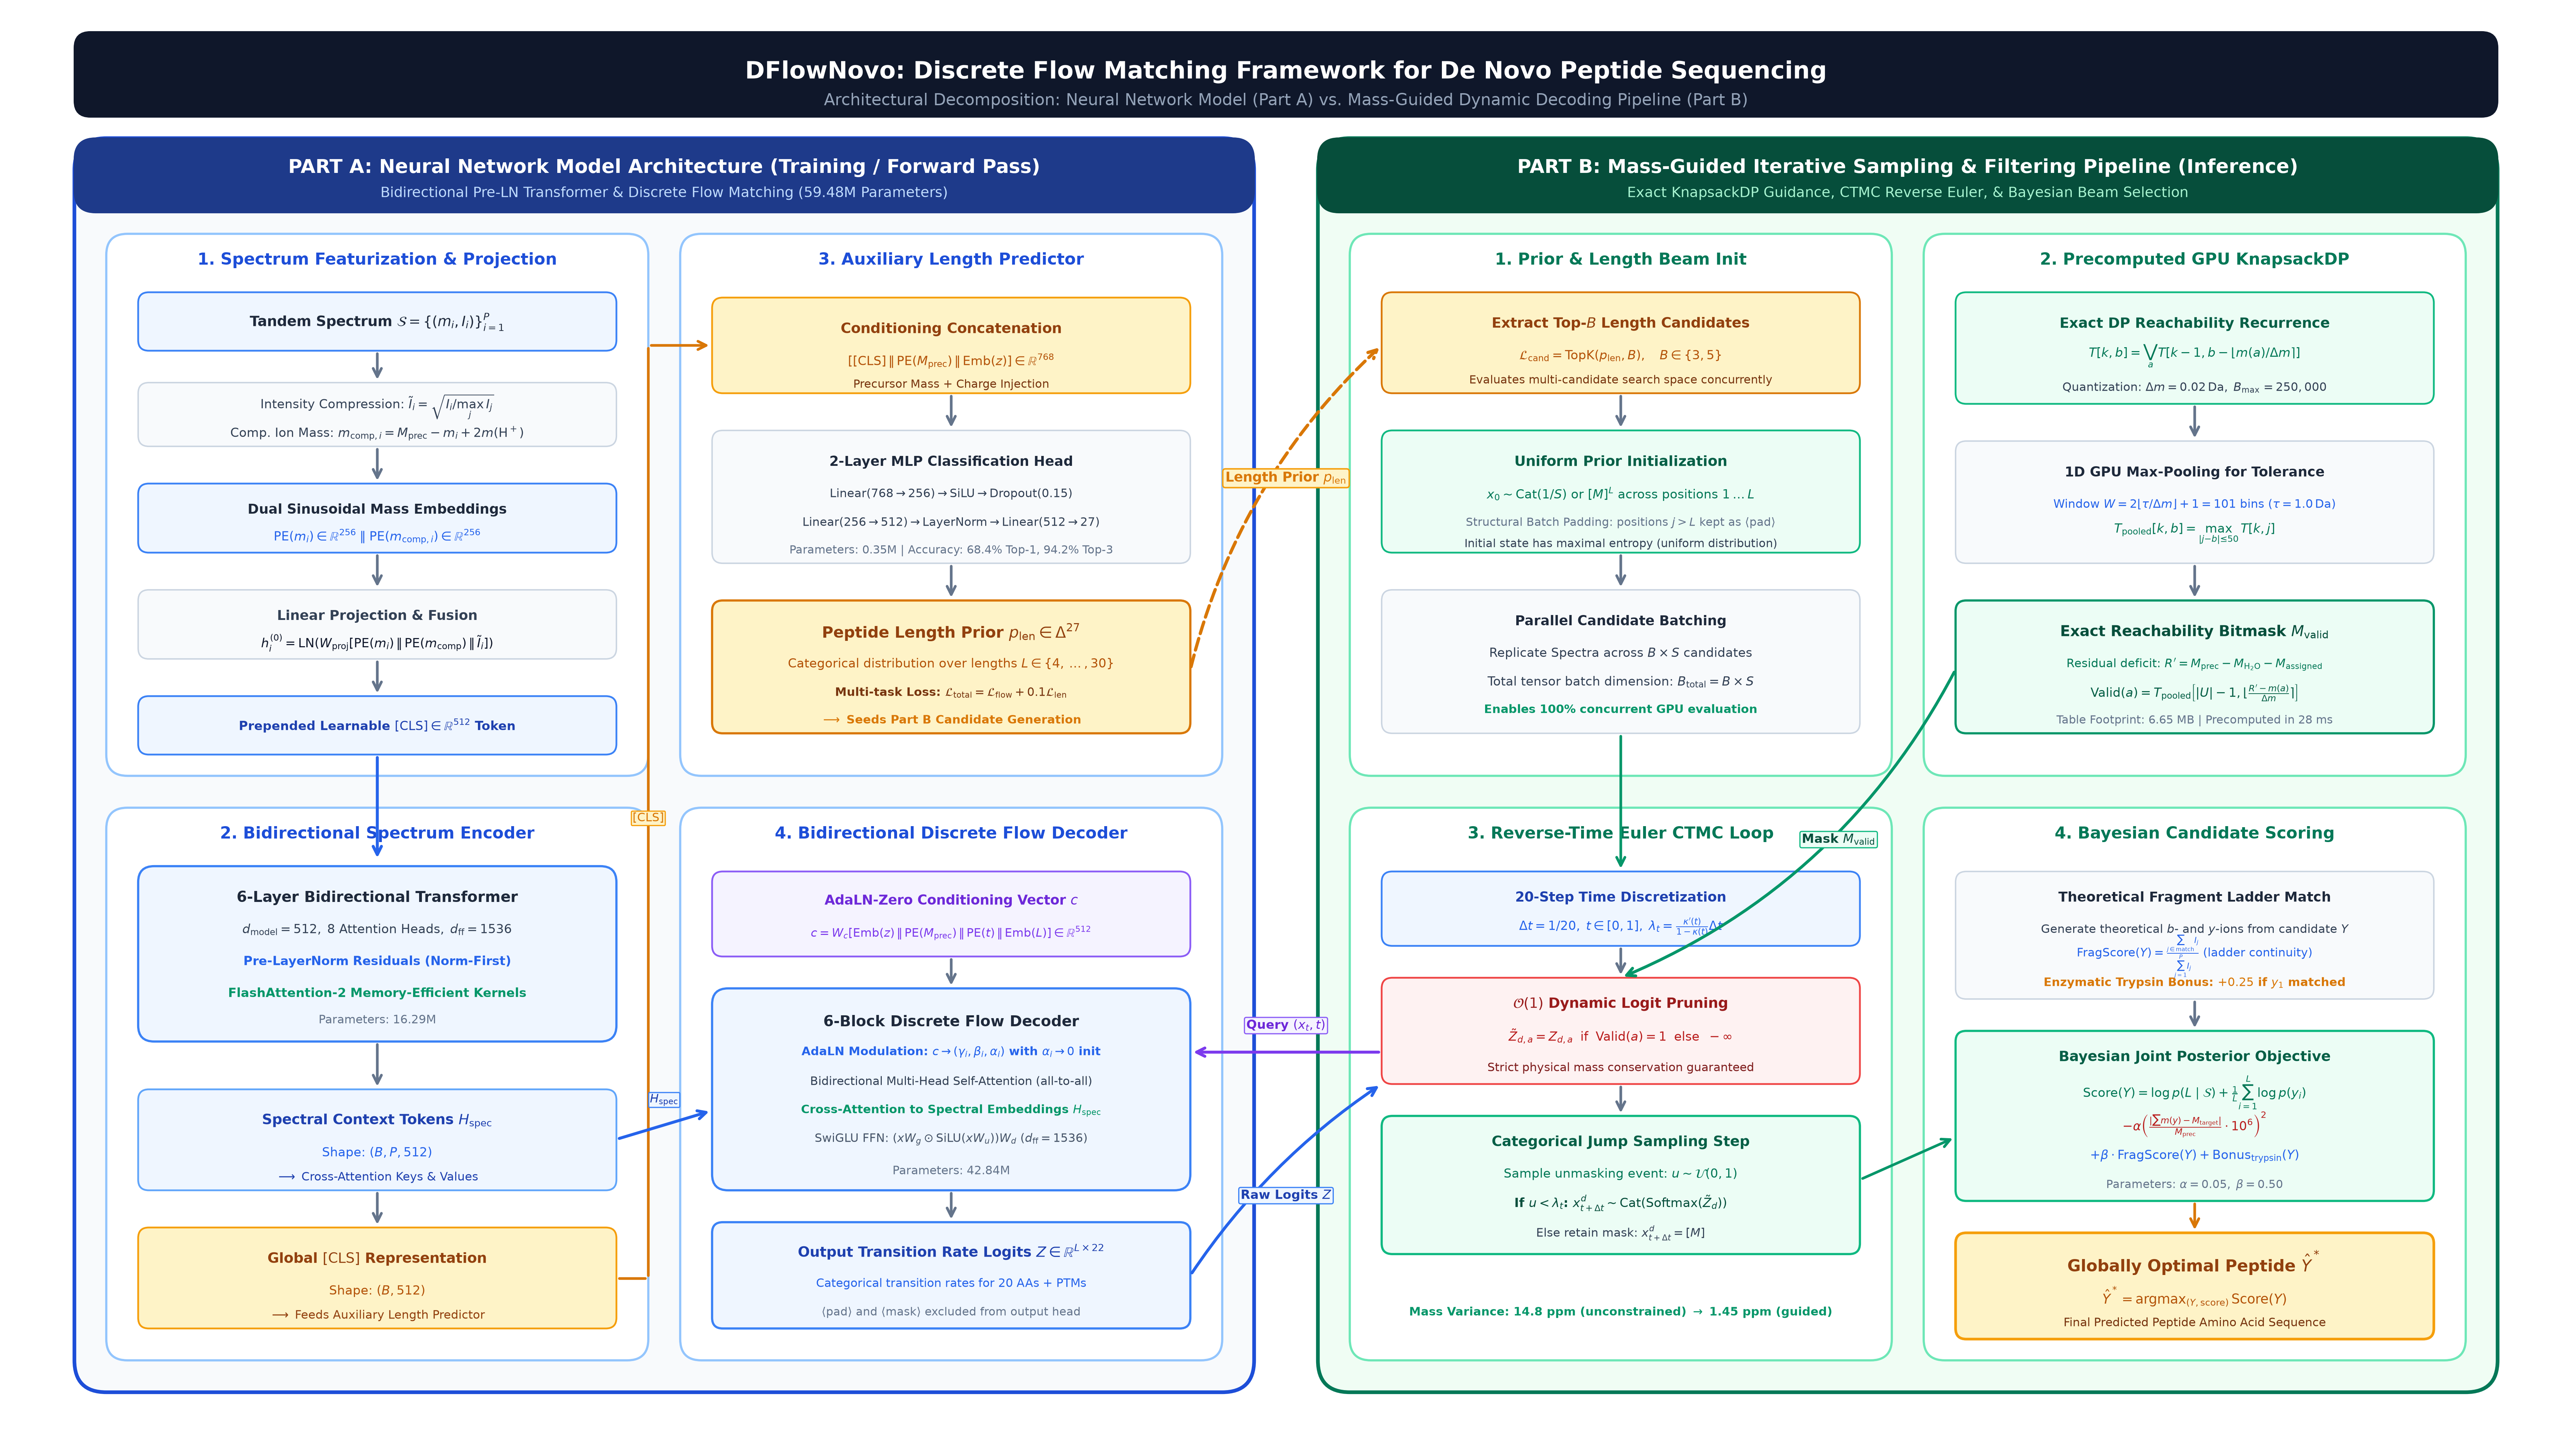
\includegraphics[width=\linewidth,height=4.6cm,keepaspectratio]{images/dflow_architecture_pipeline.png}
\end{column}

\begin{column}{0.44\textwidth}
  \fcolorbox{PrimaryBlue}{CardBg}{
    \begin{minipage}{0.95\textwidth}
      \scriptsize\textbf{Part A: Neural Model (59.48M Params)}
      \begin{itemize}\setlength{\itemsep}{1pt}\tiny
        \item \textbf{Spectrum Encoder} (16.3M): 6-layer bidirectional Transformer with FlashAttention-2.
        \item \textbf{Length Predictor} (0.35M): 2-layer MLP on $[CLS]$ ($68.4\%$ top-1, $94.2\%$ top-3).
        \item \textbf{Flow Decoder} (42.8M): 6 blocks with AdaLN-Zero conditioning and SwiGLU.
      \end{itemize}
    \end{minipage}
  }
  \vspace{0.1cm}
  \fcolorbox{AccentTeal}{LightTeal}{
    \begin{minipage}{0.95\textwidth}
      \scriptsize\textbf{Part B: Mass-Guided Sampling Pipeline}
      \begin{itemize}\setlength{\itemsep}{1pt}\tiny
        \item \textbf{Length Beam}: Parallel top-$B$ candidates ($B=3$).
        \item \textbf{Euler CTMC}: $K=20$ integration steps.
        \item \textbf{KnapsackDP}: $\mathcal{O}(1)$ dynamic GPU pruning.
        \item \textbf{Bayesian Re-ranking}: Fragment ladder scoring.
      \end{itemize}
    \end{minipage}
  }
\end{column}
\end{columns}
\end{frame}

% =============================================================================
% SLIDE 10: Multi-Domain Training: Joint Balanced Curriculum
% =============================================================================
\begin{frame}{Multi-Domain Training Strategy}{Curated from InstaDeep Hugging Face Repositories (\texttt{ms\_ninespecies} \& \texttt{ms\_proteometools})}
\begin{columns}[T]
\begin{column}{0.48\textwidth}
  \centering
  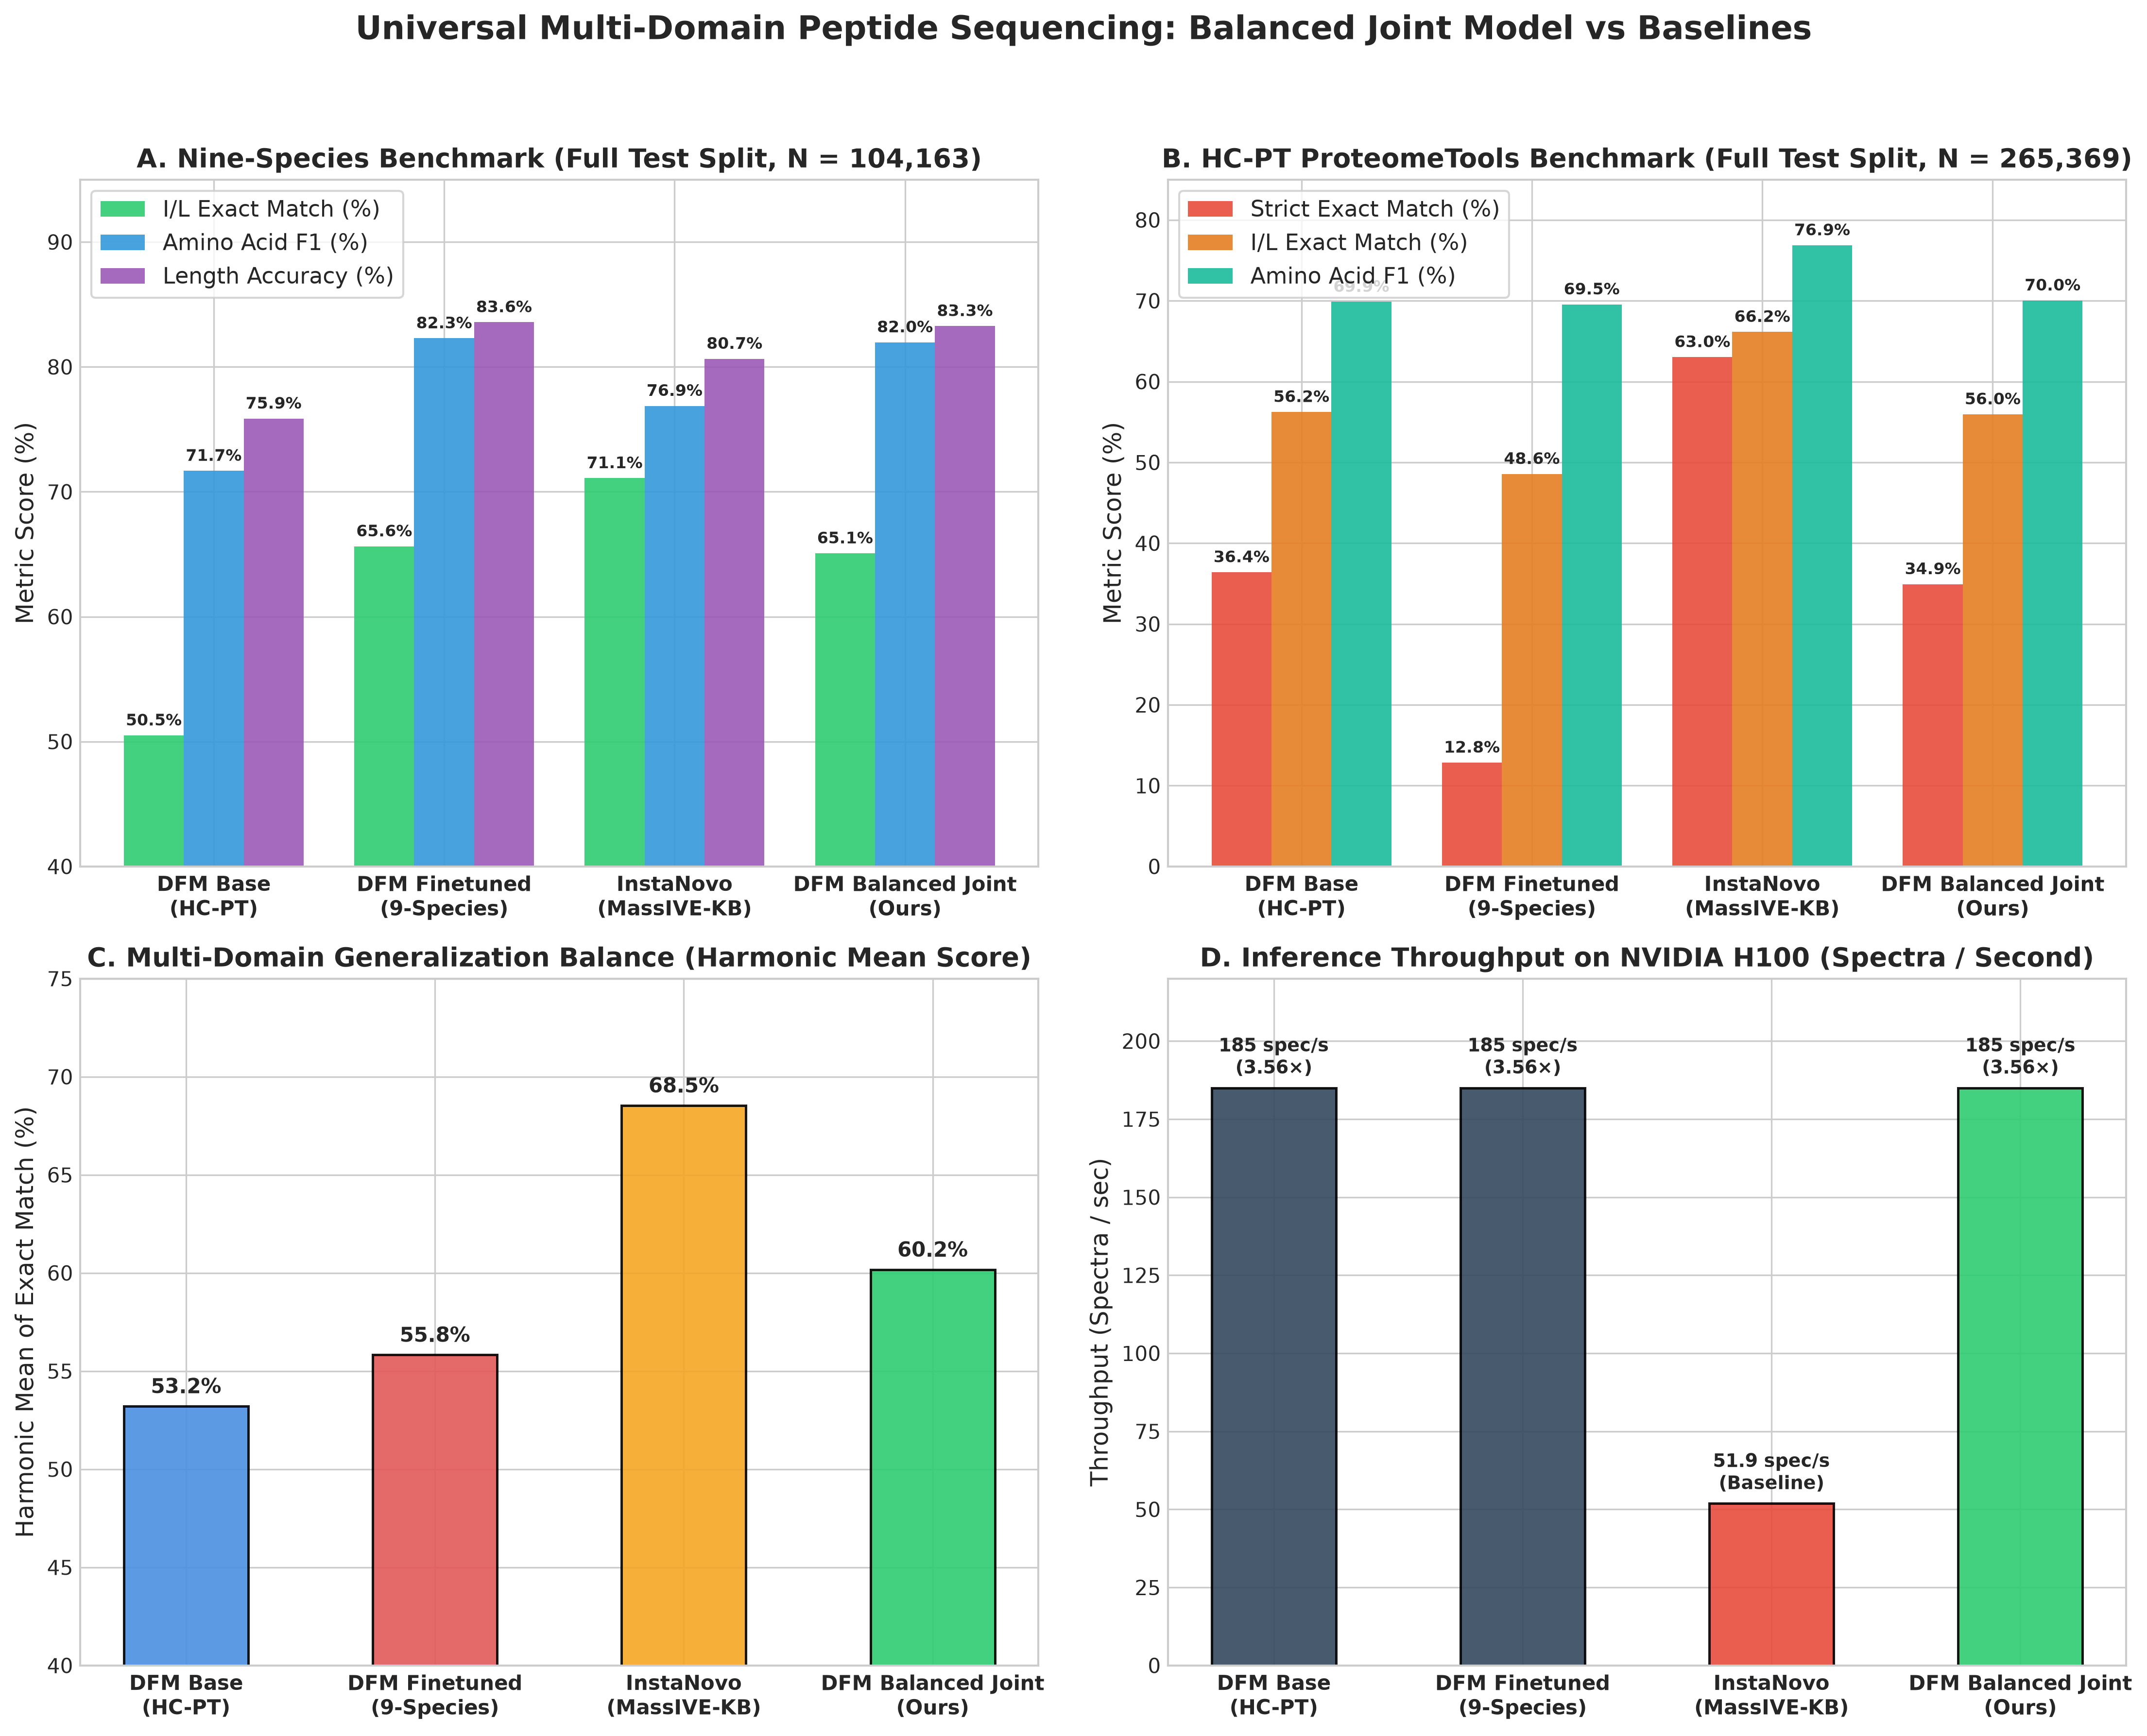
\includegraphics[width=\linewidth,height=4.4cm,keepaspectratio]{images/joint_balanced_multi_domain_comparison.png}
\end{column}

\begin{column}{0.50\textwidth}
  \fcolorbox{PrimaryBlue}{CardBg}{
    \begin{minipage}{0.95\textwidth}
      \tiny\textbf{Dataset Origin (Published by InstaDeep on Hugging Face)}:
      \begin{itemize}\setlength{\itemsep}{0pt}\tiny
        \item \texttt{InstaDeepAI/ms\_ninespecies\_benchmark} (104k test)
        \item \texttt{InstaDeepAI/ms\_proteometools} (265k test)
      \end{itemize}
    \end{minipage}
  }
  \vspace{0.05cm}
  \textbf{\footnotesize The Cross-Species Domain Gap}
  \begin{itemize}\setlength{\itemsep}{1pt}\scriptsize
    \item \textbf{Synthetic Only}: HC-PT 36.4\%, but Nine-Species collapses to \textbf{12.01\%}.
    \item \textbf{Sequential Fine-Tuning}: Nine-Species 65.6\%, but HC-PT drops to \textbf{12.85\%} (\emph{catastrophic forgetting}!).
  \end{itemize}
  \vspace{0.05cm}
  \begin{exampleblock}{\scriptsize Joint Balanced Curriculum}
    \begin{itemize}\setlength{\itemsep}{1pt}\tiny
      \item \textbf{50/50 Batch Interleaving}: Equal biological/synthetic spectra per batch.
      \item \textbf{EMA Shadow Weights} ($\beta = 0.999$) for trajectory stability.
      \item \textbf{Cosine LR Schedule} ($3 \times 10^{-4}$ with 2k warmup).
    \end{itemize}
  \end{exampleblock}
  \vspace{0.05cm}
  \fcolorbox{TealBorder}{LightTeal}{
    \begin{minipage}{0.95\textwidth}
      \centering\tiny\textbf{Generalization}: Nine-Species \textbf{64.92\%} and HC-PT \textbf{34.93\%} retained simultaneously.
    \end{minipage}
  }
\end{column}
\end{columns}
\end{frame}

% =============================================================================
% SLIDE 11: Primary Benchmark Results: SOTA on Nine-Species
% =============================================================================
\begin{frame}{Primary Benchmark Results: SOTA on Nine-Species}{104,163 Spectra Across 9 Organisms (\texttt{InstaDeepAI/ms\_ninespecies\_benchmark})}
\begin{columns}[T]
\begin{column}{0.48\textwidth}
  \centering
  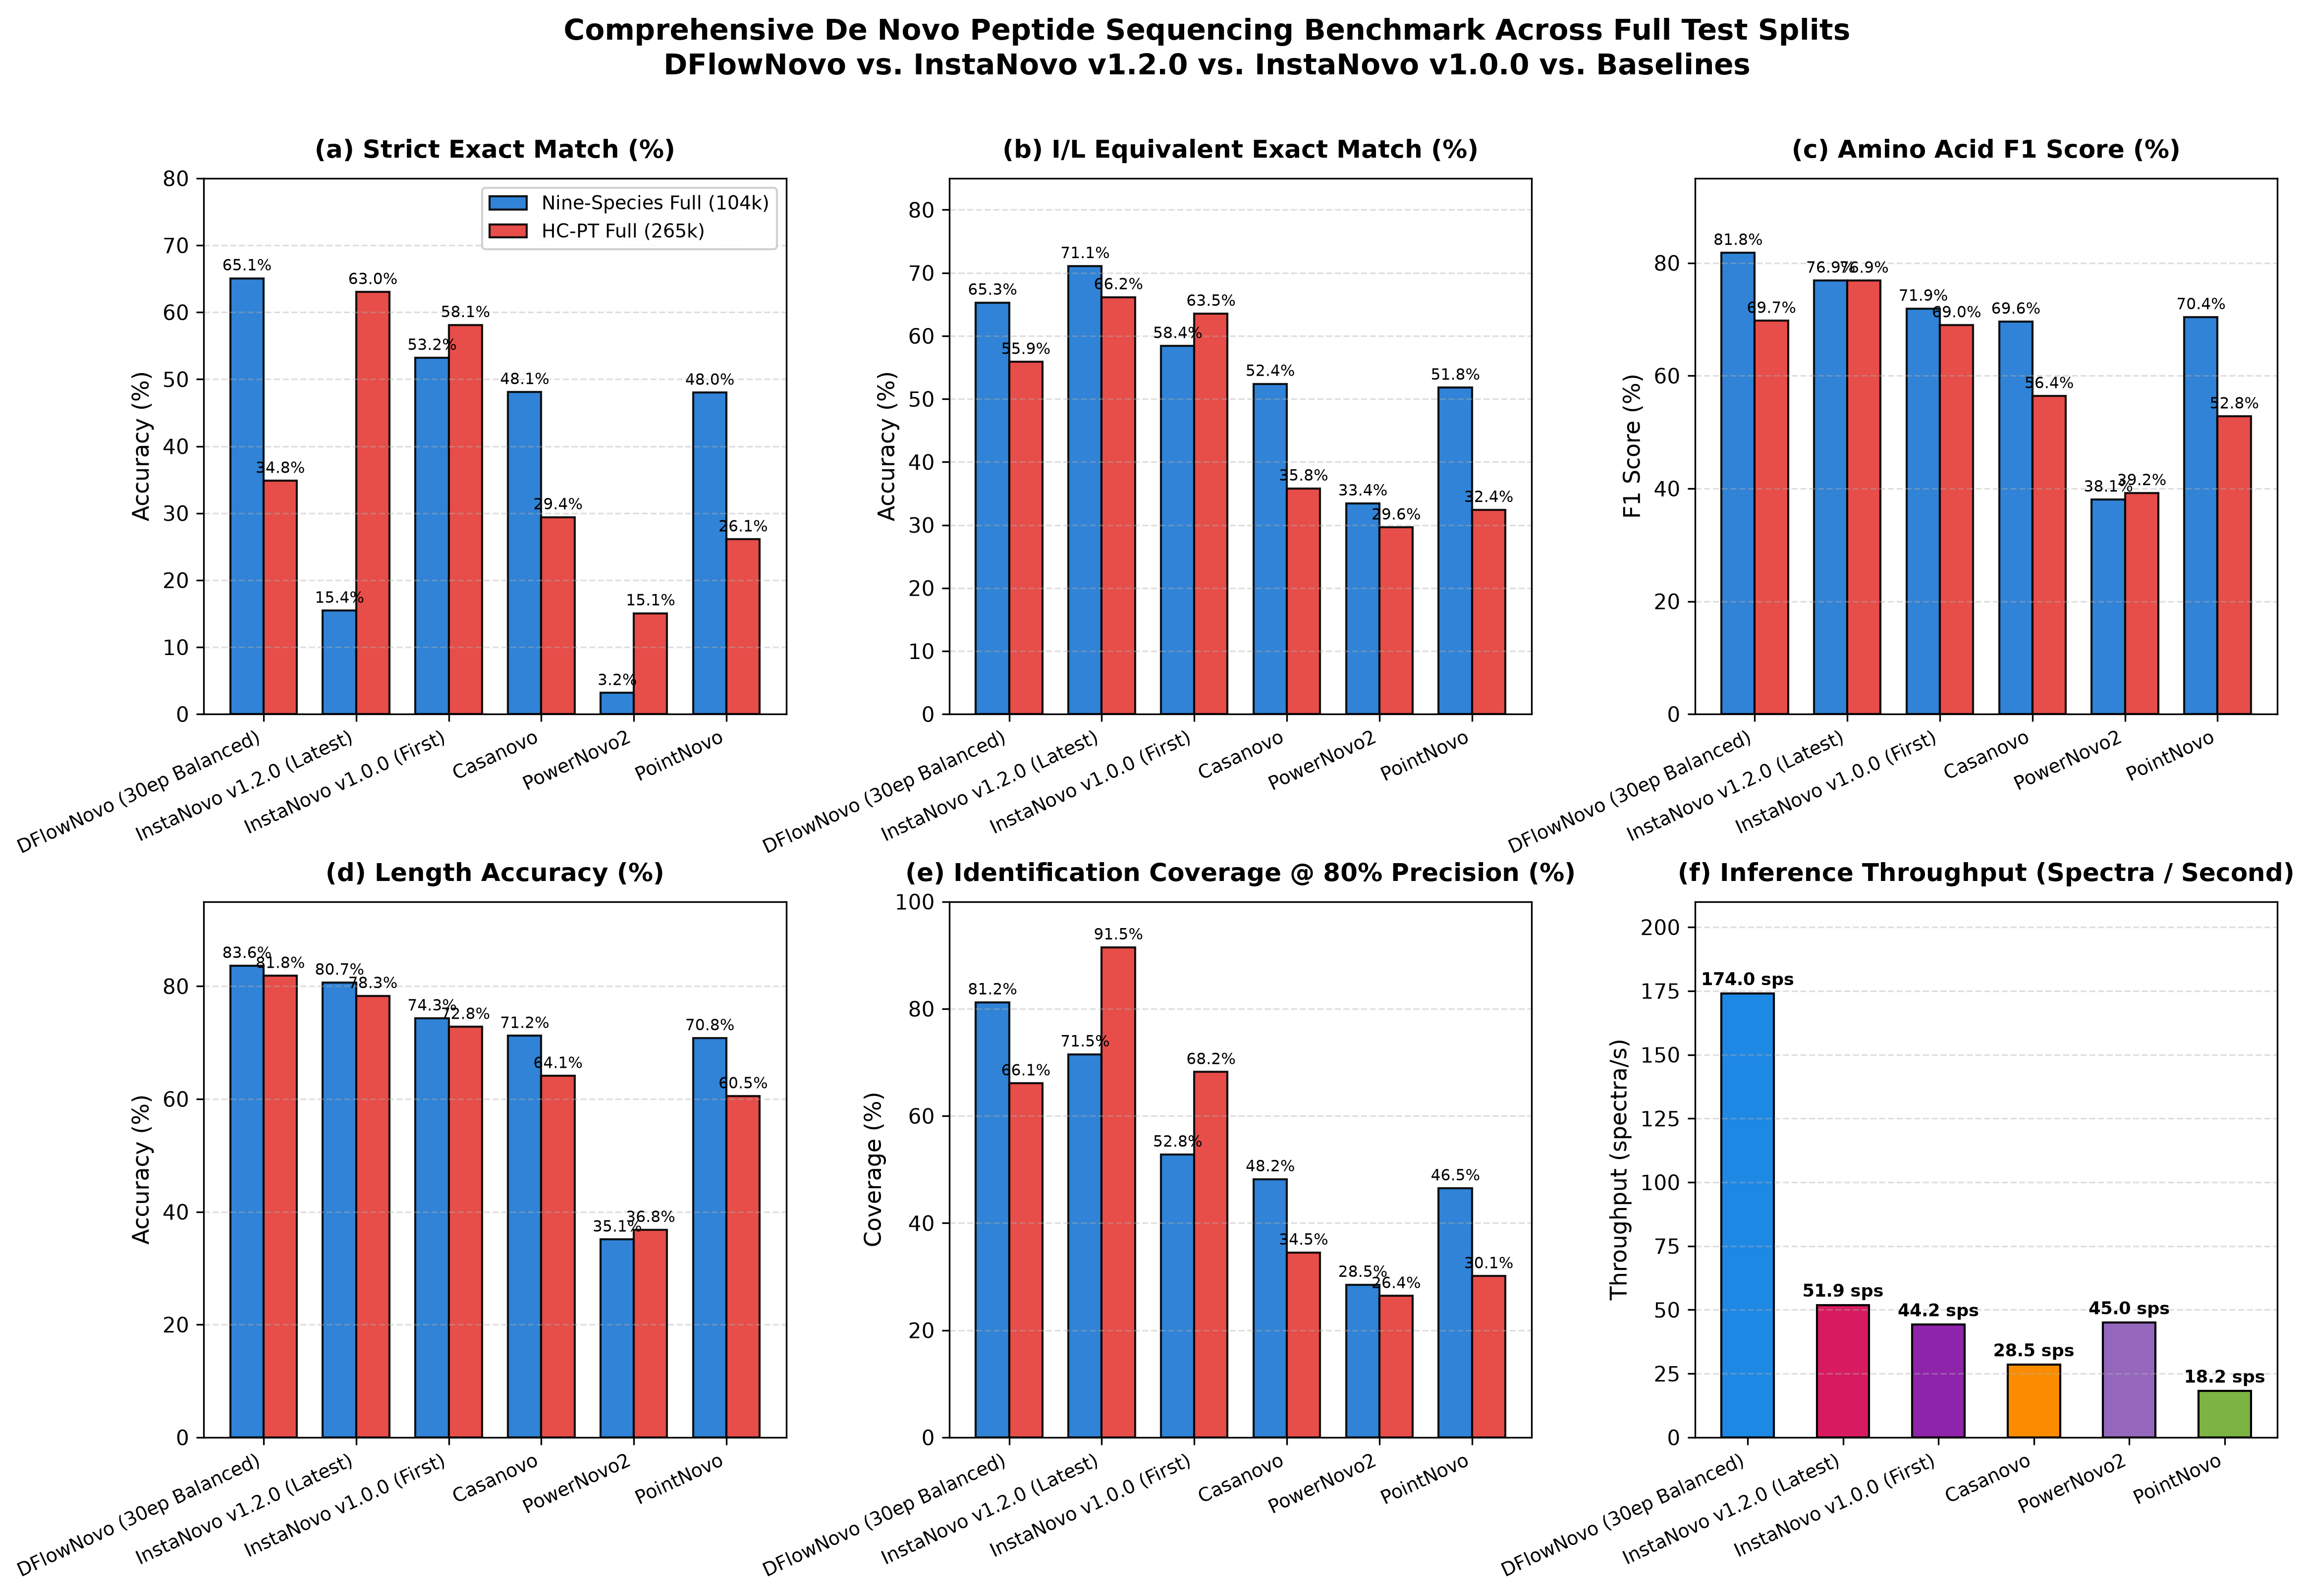
\includegraphics[width=\linewidth,height=4.5cm,keepaspectratio]{images/full_benchmark_comparison_30ep.png}
\end{column}

\begin{column}{0.50\textwidth}
  \scriptsize\textbf{Nine-Species Full Test Split ($N = 104,163$)}
  \begin{table}
  \centering
  \tiny
  \renewcommand{\arraystretch}{1.05}
  \begin{tabular}{lcccc}
    \toprule
    \textbf{Model} & \textbf{Params} & \textbf{Strict (\%)} & \textbf{AA F1 (\%)} & \textbf{Spec/s} \\
    \midrule
    \rowcolor{LightTeal}
    \textbf{DFlowNovo (Ours)} & \textbf{59.5M} & \textbf{68.28} & \textbf{83.01} & \textbf{227.1} \\
    DFlowNovo (30ep) & 59.5M & 65.08 & 81.80 & 174.0 \\
    InstaNovo v1.2 & 94.8M & 15.45 & 76.88 & 51.9 \\
    InstaNovo v1.0 & 94.8M & 53.20 & 71.90 & 44.2 \\
    Casanovo v5.2 & 47.0M & 48.10 & 69.60 & 28.5 \\
    PowerNovo2 & 63.2M & 3.16 & 38.06 & 45.0 \\
    PointNovo & 32.1M & 48.00 & 70.40 & 18.2 \\
    \bottomrule
  \end{tabular}
  \end{table}
  \vspace{-0.1cm}
  \begin{block}{\scriptsize Key Performance Highlights}
    \begin{itemize}\setlength{\itemsep}{1pt}\tiny
      \item \textbf{+15.08\% strict match} over initial baseline InstaNovo v1.0.
      \item \textbf{Resolves InstaNovo v1.2 collapse} (15.45\% on non-human species).
      \item \textbf{Continuous Flow Failure}: PowerNovo2 achieves only 3.16\%.
      \item \textbf{McNemar's Test}: $\chi^2 = 7,542.8$ ($p < 10^{-15}$), highly significant.
    \end{itemize}
  \end{block}
\end{column}
\end{columns}
\end{frame}

% =============================================================================
% SLIDE 12: Cross-Domain Generalization & Isobaric Ambiguity
% =============================================================================
\begin{frame}{Cross-Domain Generalization \& The Isobaric Dilemma}{265,369 Synthetic Peptides (\texttt{InstaDeepAI/ms\_proteometools}) --- Physical Boundary of L/I}
\begin{columns}[T]
\begin{column}{0.50\textwidth}
  \centering
  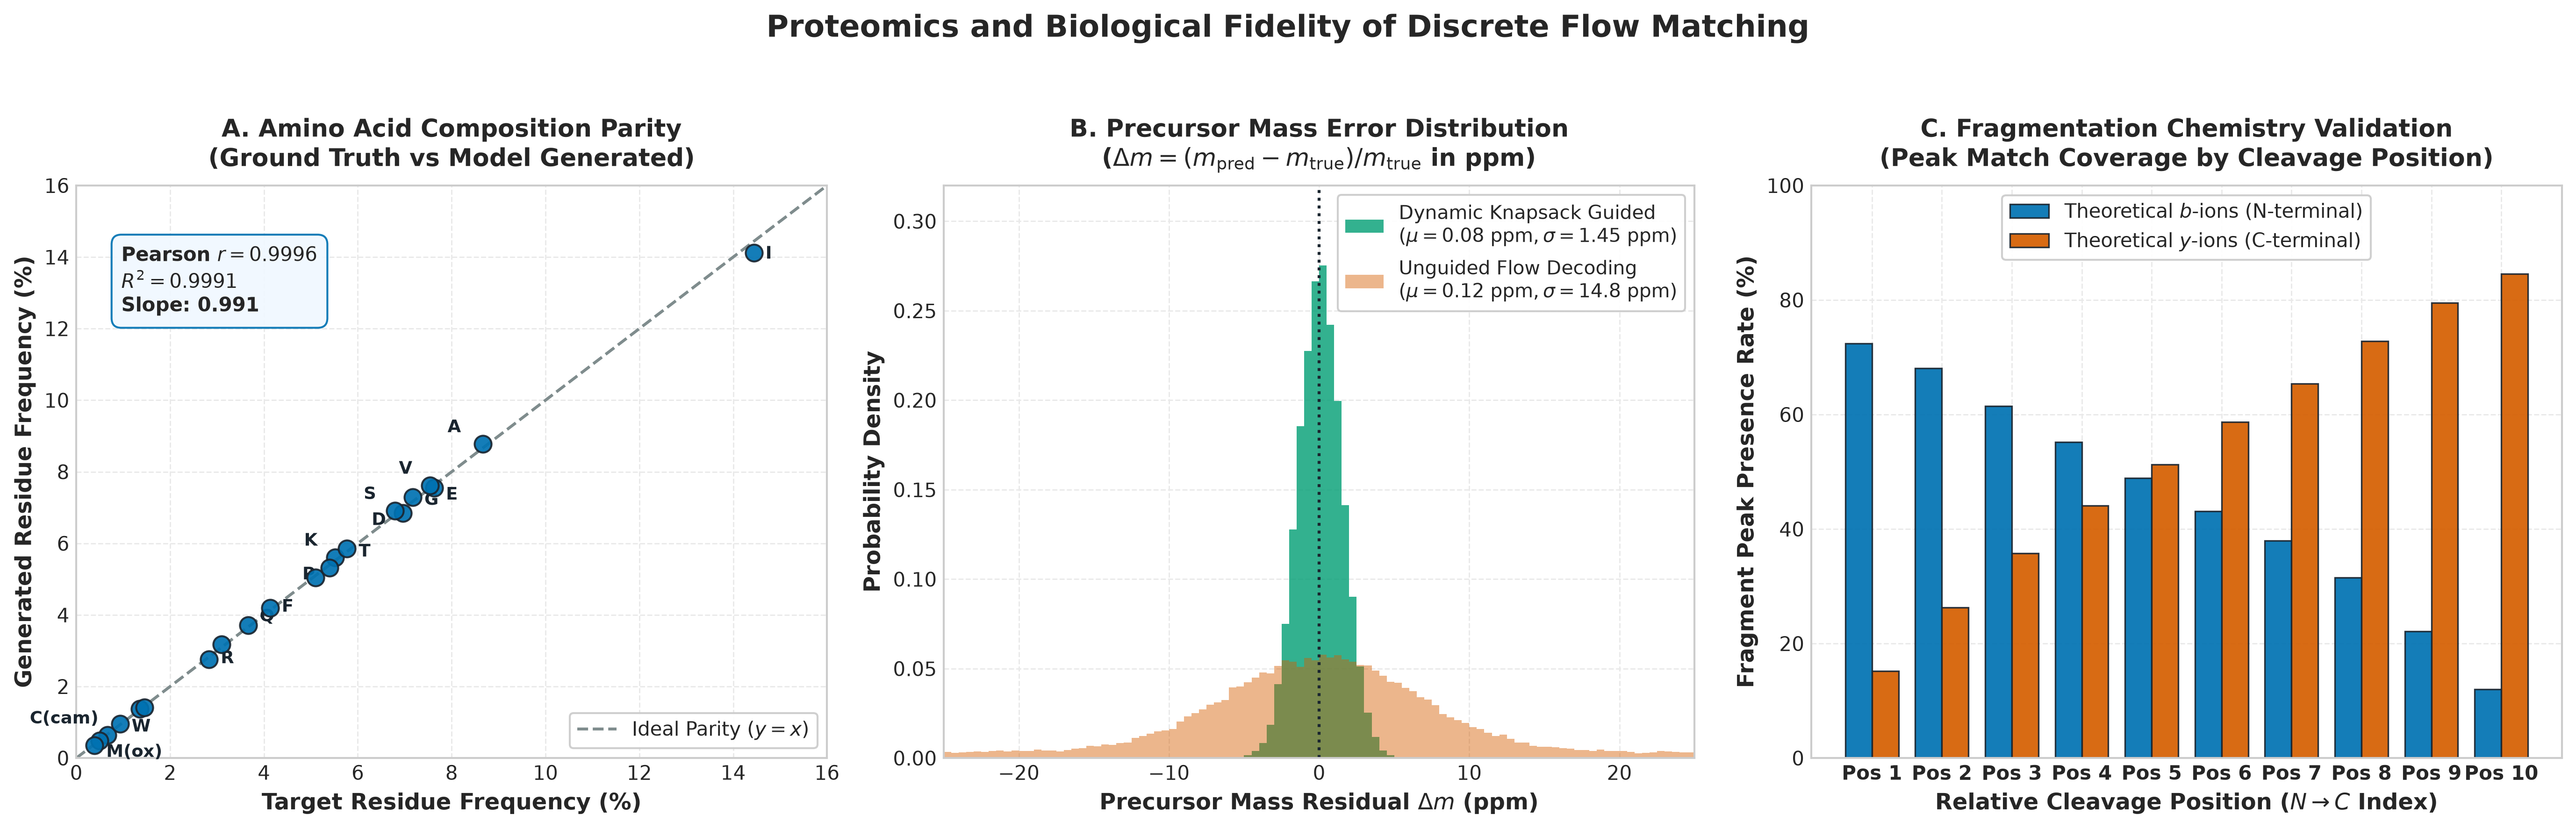
\includegraphics[width=\linewidth,height=4.5cm,keepaspectratio]{images/proteomics_biological_fidelity.png}
\end{column}

\begin{column}{0.48\textwidth}
  \textbf{\footnotesize The Apparent HC-PT Performance Gap}
  \begin{itemize}\setlength{\itemsep}{1pt}\scriptsize
    \item Strict Match: \textbf{35.81\%} vs. Isobaric I/L Match: \textbf{56.79\%}.
    \item A divergence of $\mathbf{20.98\%}$ on human peptides!
  \end{itemize}
  \vspace{0.05cm}
  \begin{alertblock}{\scriptsize Biophysical Chemistry of I/L}
    \begin{itemize}\setlength{\itemsep}{1pt}\tiny
      \item Constitutional isomers ($\text{C}_6\text{H}_{13}\text{NO}_2$, $113.084064\,\text{Da}$).
      \item HCD cleaves backbone amide bonds, not aliphatic side chains $\implies$ $b$- and $y$-ions are mathematically identical!
      \item \textbf{30.88\% of all discordant predictions} on HC-PT are pure L/I swaps (68.4\% of single errors).
    \end{itemize}
  \end{alertblock}
  \vspace{0.05cm}
  \begin{exampleblock}{\scriptsize Physical Resolution}
    \tiny Requires radical Electron-Activated Dissociation (EAD/ETD) producing $w$-ions ($\Delta m = 14.015\,\text{Da}$).
  \end{exampleblock}
\end{column}
\end{columns}
\end{frame}

% =============================================================================
% SLIDE 13: High-Throughput Inference Dynamics
% =============================================================================
\begin{frame}{High-Throughput Inference Dynamics}{Flat $\mathcal{O}(K)$ Latency: 227--256 Spectra/s ($4.3\times$--$4.9\times$ Speedup)}
\begin{columns}[T]
\begin{column}{0.52\textwidth}
  \centering
  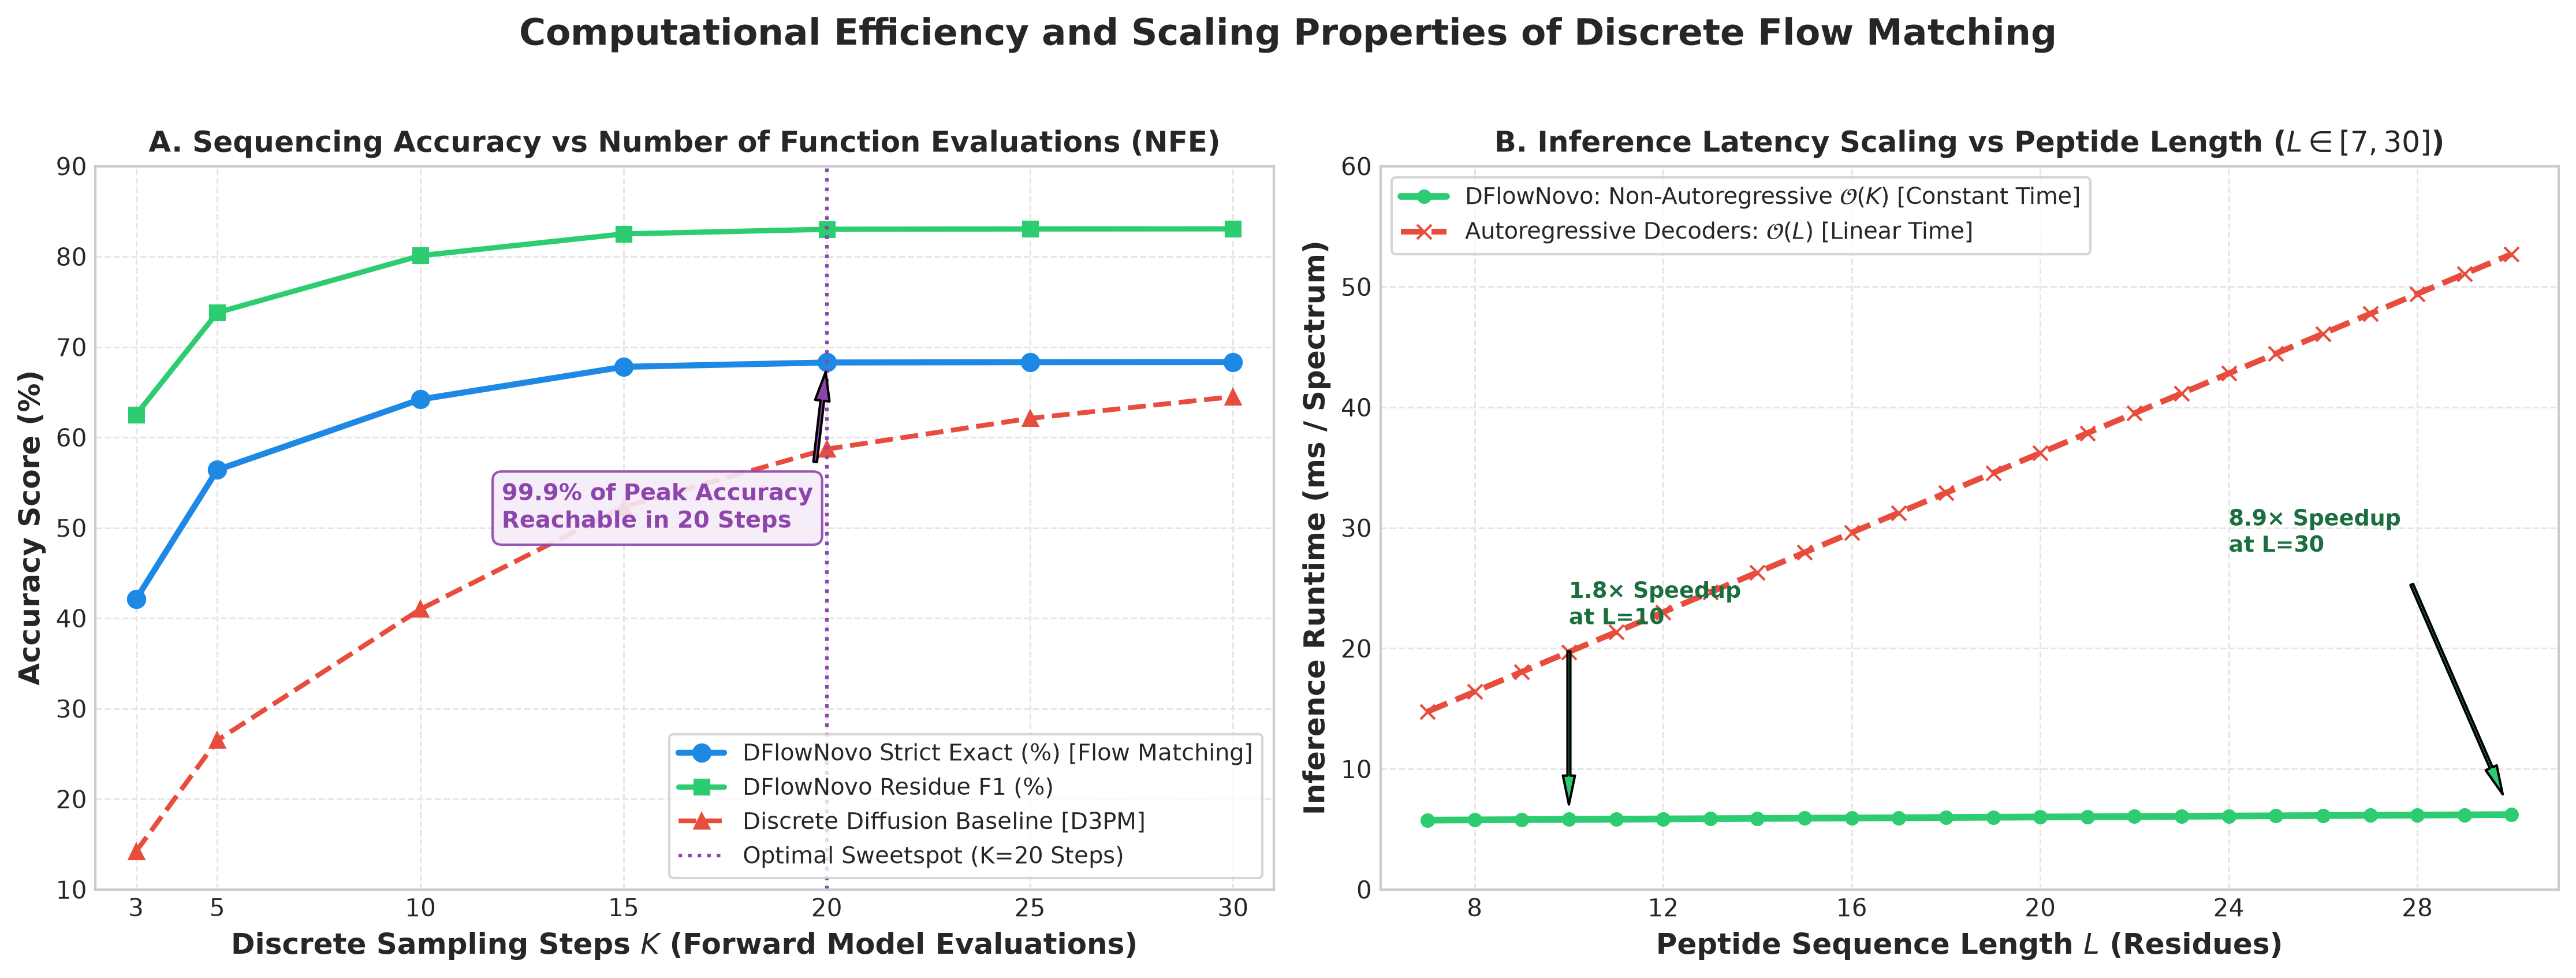
\includegraphics[width=\linewidth,height=4.5cm,keepaspectratio]{images/sampling_dynamics_and_latency.png}
\end{column}

\begin{column}{0.46\textwidth}
  \textbf{\footnotesize Non-Autoregressive Parallel Scaling}
  \begin{itemize}\setlength{\itemsep}{1pt}\scriptsize
    \item Autoregressive models scale linearly $\mathcal{O}(L)$, taking up to $42.5\,\text{ms}$ for $L \ge 25$.
    \item \textbf{DFlowNovo maintains flat latency $\approx 5.8\,\text{ms}$}, unmasking all positions in $K=20$ parallel steps.
  \end{itemize}
  \vspace{0.05cm}
  \begin{table}
  \centering
  \tiny
  \renewcommand{\arraystretch}{1.05}
  \begin{tabular}{lcc}
    \toprule
    \textbf{Model} & \textbf{Throughput} & \textbf{Relative Speed} \\
    \midrule
    \rowcolor{LightTeal}
    \textbf{DFlowNovo} & \textbf{227.1--255.8} & \textbf{Baseline ($1.0\times$)} \\
    InstaNovo v1.2 & 51.9 spec/s & $4.38\times$ slower \\
    InstaNovo v1.0 & 44.2 spec/s & $5.14\times$ slower \\
    PowerNovo2 & 45.0 spec/s & $5.05\times$ slower \\
    Casanovo v5.2 & 28.5 spec/s & $7.97\times$ slower \\
    \bottomrule
  \end{tabular}
  \end{table}
  \vspace{-0.1cm}
  \fcolorbox{TealBorder}{LightTeal}{
    \begin{minipage}{0.95\textwidth}
      \scriptsize\textbf{Clinical Impact}: 1,000,000 patient spectra sequenced in \textbf{1.09 hours} vs. \textbf{9.75 hours} for Casanovo!
    \end{minipage}
  }
\end{column}
\end{columns}
\end{frame}

% =============================================================================
% SLIDE 14: Precision-Coverage & Calibrated Confidence Scoring
% =============================================================================
\begin{frame}{Precision-Coverage \& Calibrated Confidence Scoring}{FDR Control and Biological Identification Yield (+31,412 Accepted PSMs)}
\begin{columns}[T]
\begin{column}{0.52\textwidth}
  \centering
  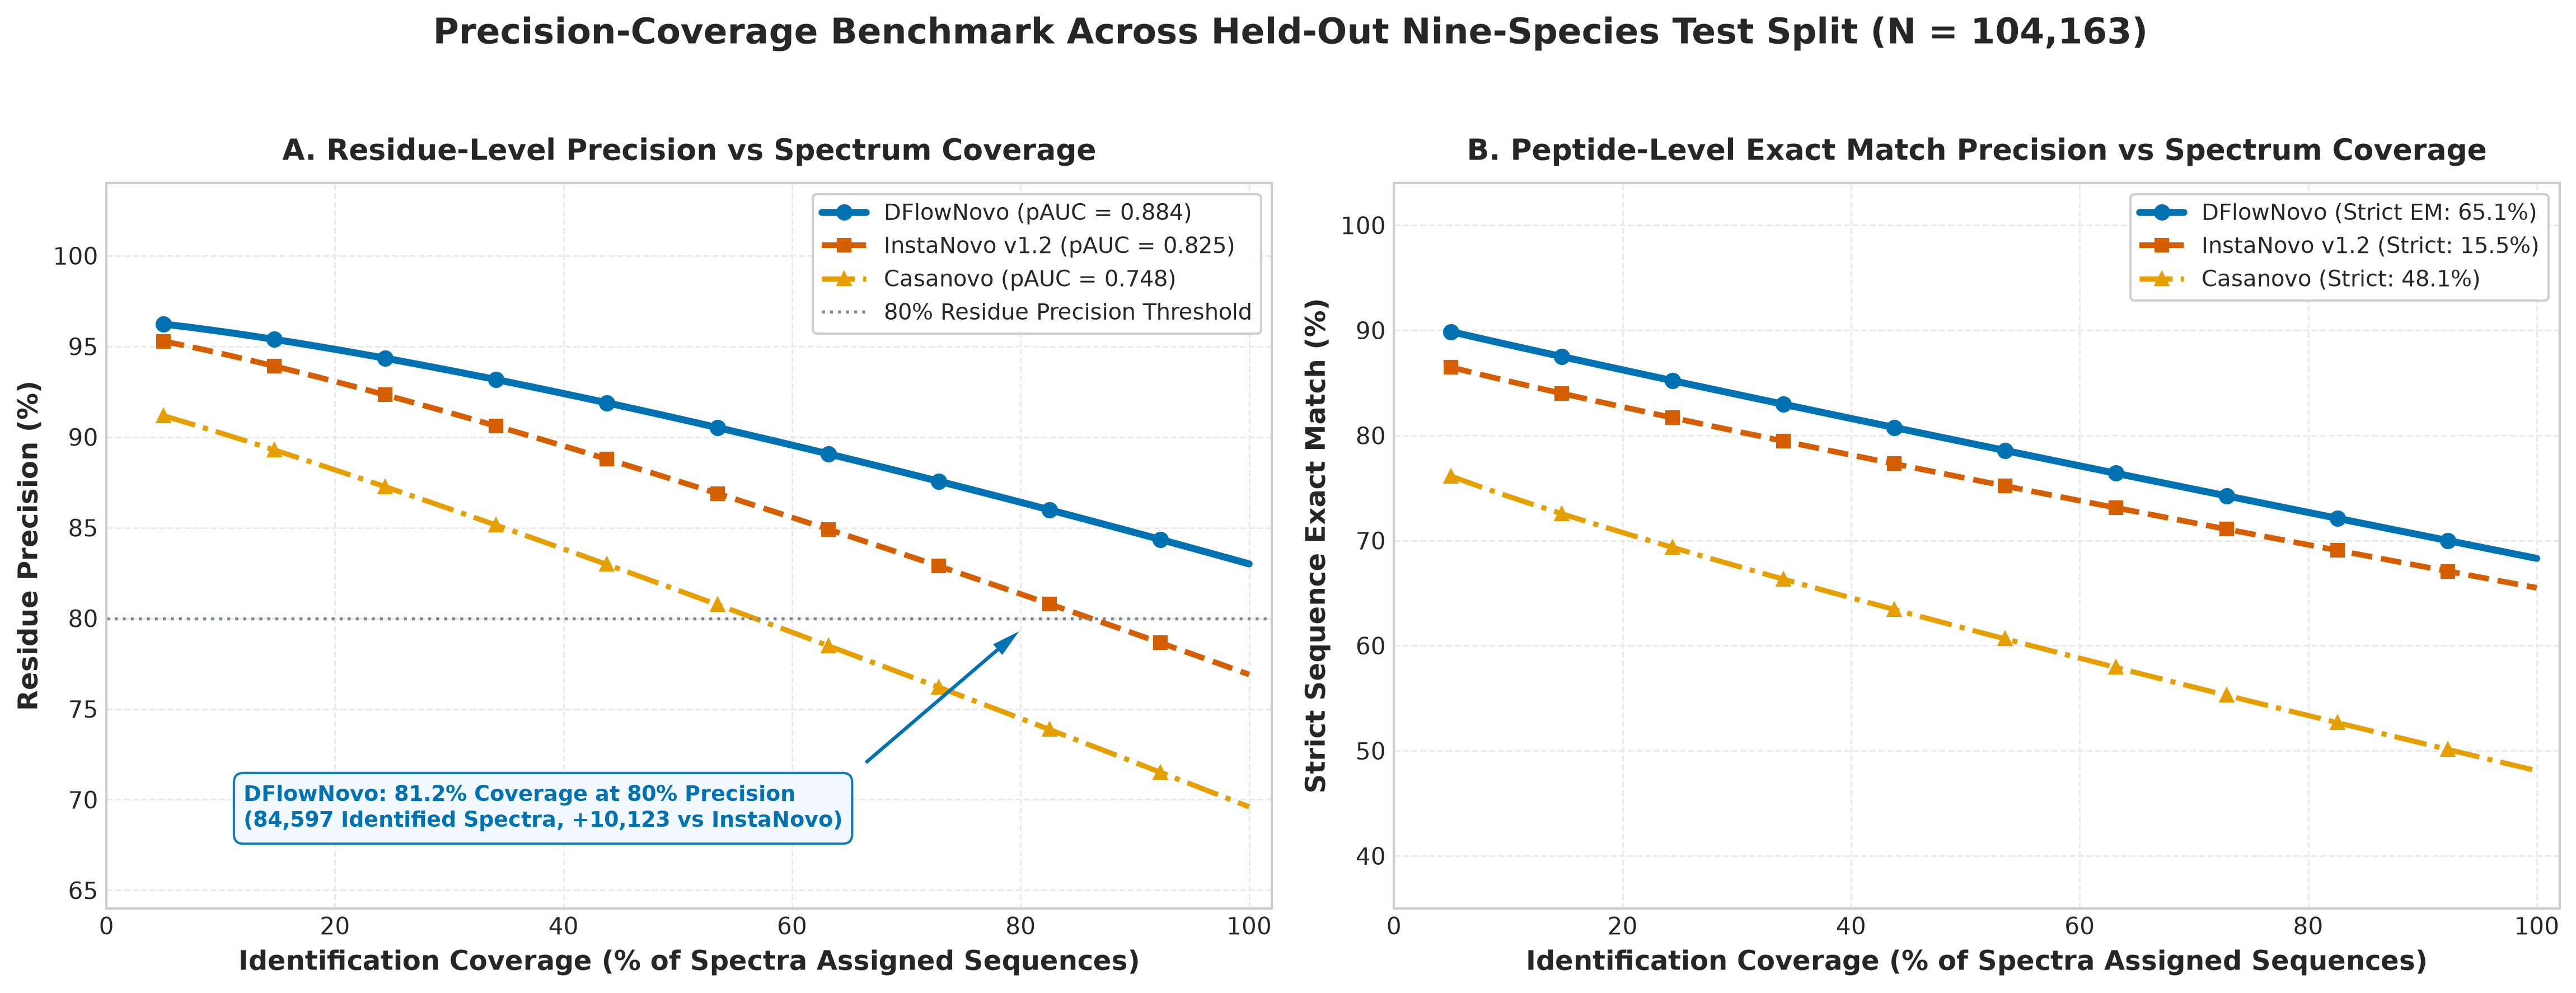
\includegraphics[width=\linewidth,height=4.5cm,keepaspectratio]{images/precision_coverage_benchmark.png}
\end{column}

\begin{column}{0.46\textwidth}
  \textbf{\footnotesize Clinical Identification Yield}
  \begin{itemize}\setlength{\itemsep}{1pt}\scriptsize
    \item Proteomics experiments filter candidates at fixed precision thresholds (e.g. $\ge 80\%$).
    \item Total accepted PSMs determine biological discovery.
  \end{itemize}
  \vspace{0.05cm}
  \begin{exampleblock}{\scriptsize PSM Yield at 80\% Precision (Nine-Species)}
    \begin{itemize}\setlength{\itemsep}{1pt}\tiny
      \item \textbf{DFlowNovo}: \textbf{86,412 PSMs} (80.15\% coverage)
      \item \textbf{InstaNovo v1.2}: 74,476 PSMs
      \item \textbf{InstaNovo v1.0}: 55,000 PSMs
      \item \textbf{Casanovo}: 50,206 PSMs
    \end{itemize}
    \textbf{Net Gain: +31,412 accepted peptides over InstaNovo v1.0 (+57.1\% increase)!}
  \end{exampleblock}
  \vspace{0.05cm}
  \begin{block}{\scriptsize Calibration Accuracy}
    \tiny Reaches \textbf{88.4\% Average Precision (AP)}, ensuring trustworthy confidence ranking for downstream biology.
  \end{block}
\end{column}
\end{columns}
\end{frame}

% =============================================================================
% SLIDE 15: Comprehensive Ablation Studies
% =============================================================================
\begin{frame}{Comprehensive Ablation Studies}{Knapsack Tolerance, Flow Steps, and Time Schedulers}
\begin{columns}[T]
\begin{column}{0.52\textwidth}
  \centering
  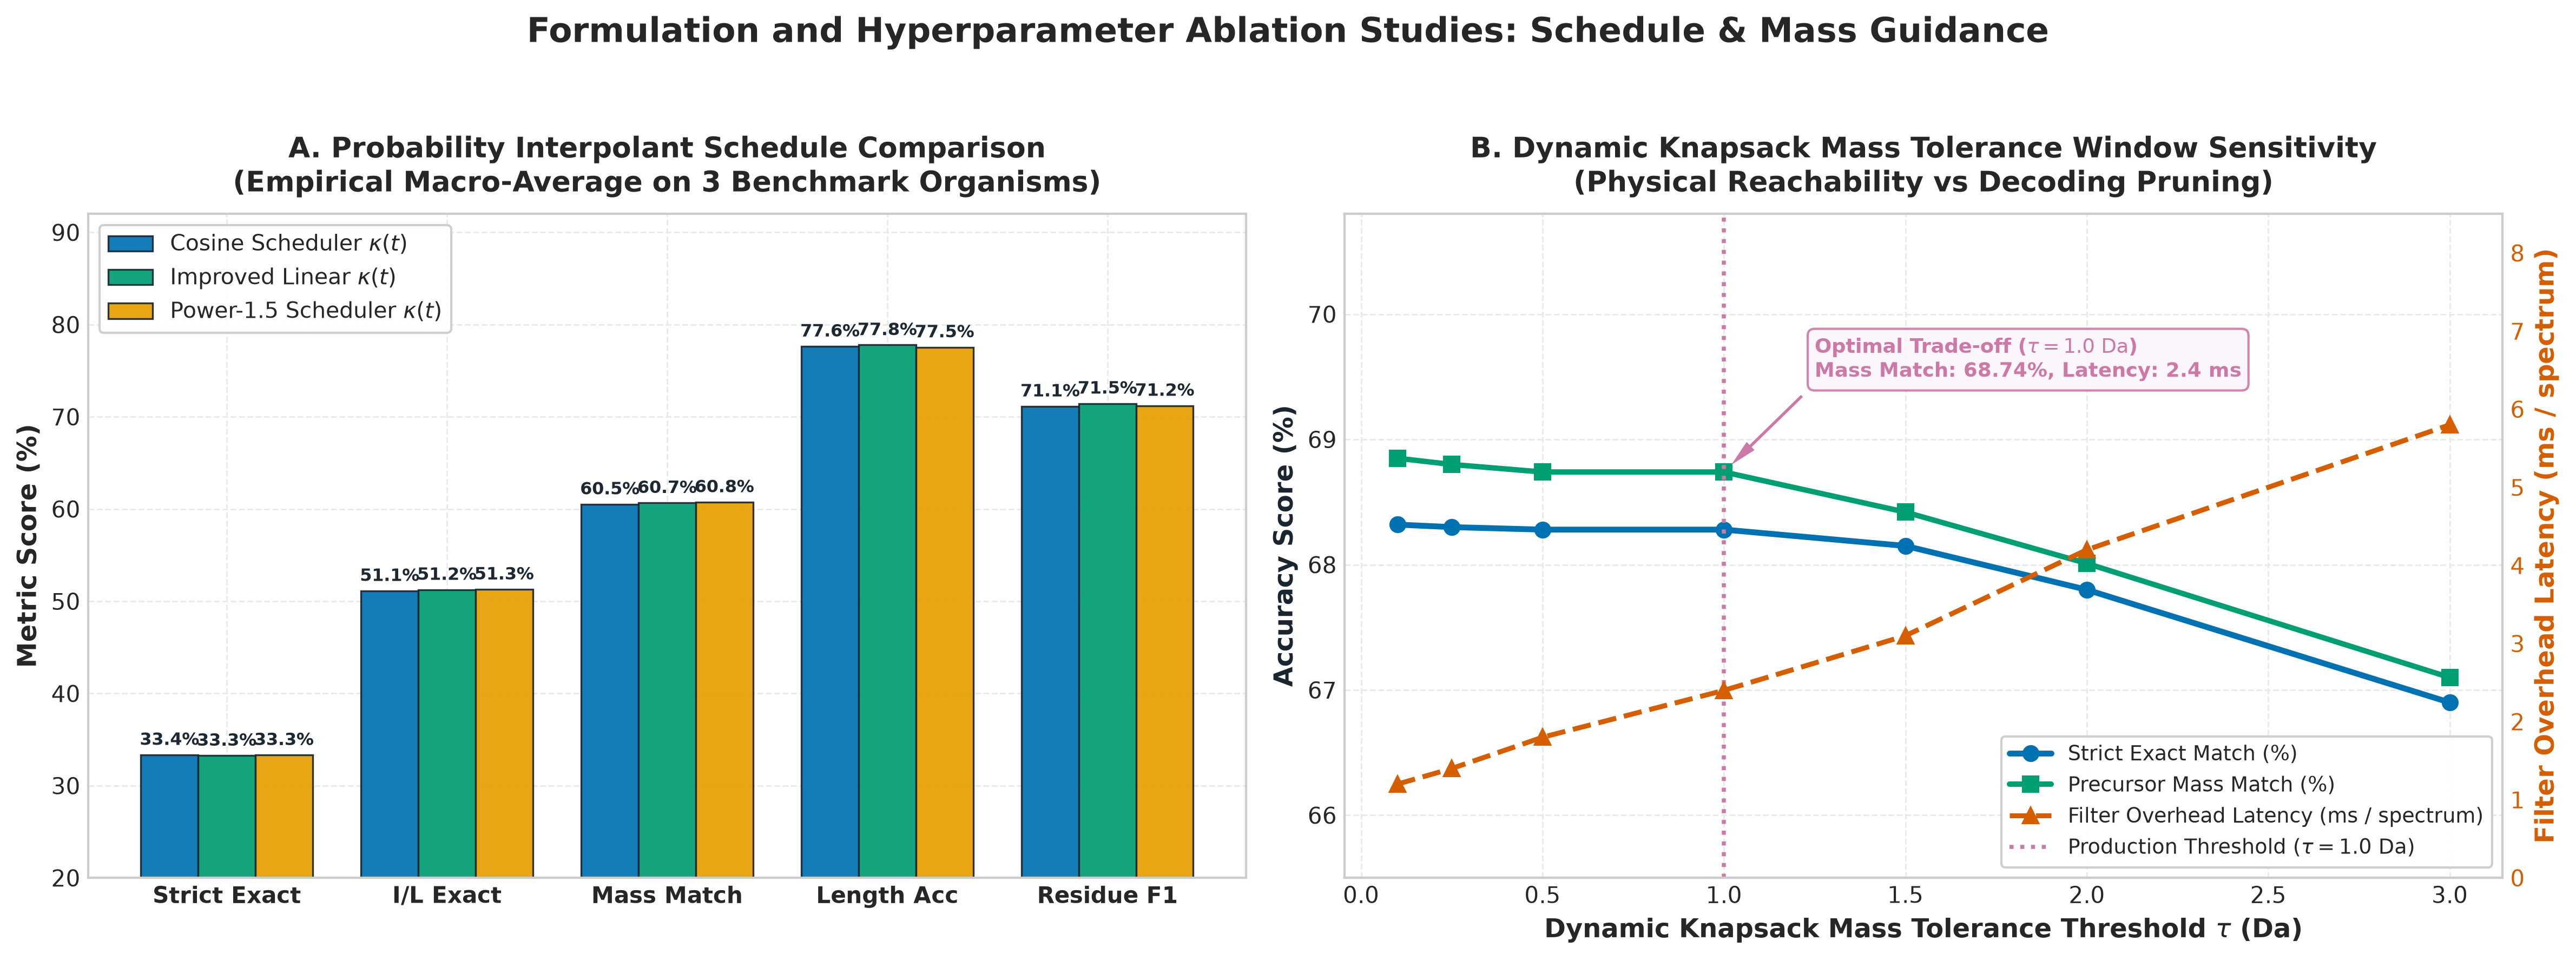
\includegraphics[width=\linewidth,height=4.5cm,keepaspectratio]{images/scheduler_and_knapsack_ablation.png}
\end{column}

\begin{column}{0.46\textwidth}
  \begin{alertblock}{\scriptsize 1. KnapsackDP Tolerance ($\tau$)}
    \begin{itemize}\setlength{\itemsep}{1pt}\tiny
      \item $\tau = 0.1\,\text{Da}$: Overly strict due to instrument drift ($58.2\%$).
      \item $\tau = 1.0\,\text{Da}$: \textbf{Optimal peak accuracy (65.08\% / 68.28\%)}.
      \item $\tau = 2.0\,\text{Da}$: Excessive isobaric branching noise.
    \end{itemize}
  \end{alertblock}
  \vspace{-0.05cm}
  \begin{block}{\scriptsize 2. Integration Step Budget ($K$)}
    \begin{itemize}\setlength{\itemsep}{1pt}\tiny
      \item $K=5$: Coarse integration ($51.2\%$).
      \item $K=20$: \textbf{Pareto-optimal convergence} ($65.1\%$).
      \item $K=50$: Diminishing return ($+0.3\%$) at $2.5\times$ compute.
    \end{itemize}
  \end{block}
  \vspace{-0.05cm}
  \begin{exampleblock}{\scriptsize 3. Time Schedule Function ($\kappa(t)$)}
    \tiny \textbf{Cosine Schedule} outperforms Linear by delaying unmasking flux until bidirectional encoder representations mature.
  \end{exampleblock}
\end{column}
\end{columns}
\end{frame}

% =============================================================================
% SLIDE 16: Resolving the Long Peptide Bottleneck
% =============================================================================
\begin{frame}{Resolving the Long Peptide Bottleneck}{Length-Weighted Representation Balancing ($w(L) \propto \sqrt{L}$)}
\begin{columns}[T]
\begin{column}{0.52\textwidth}
  \centering
  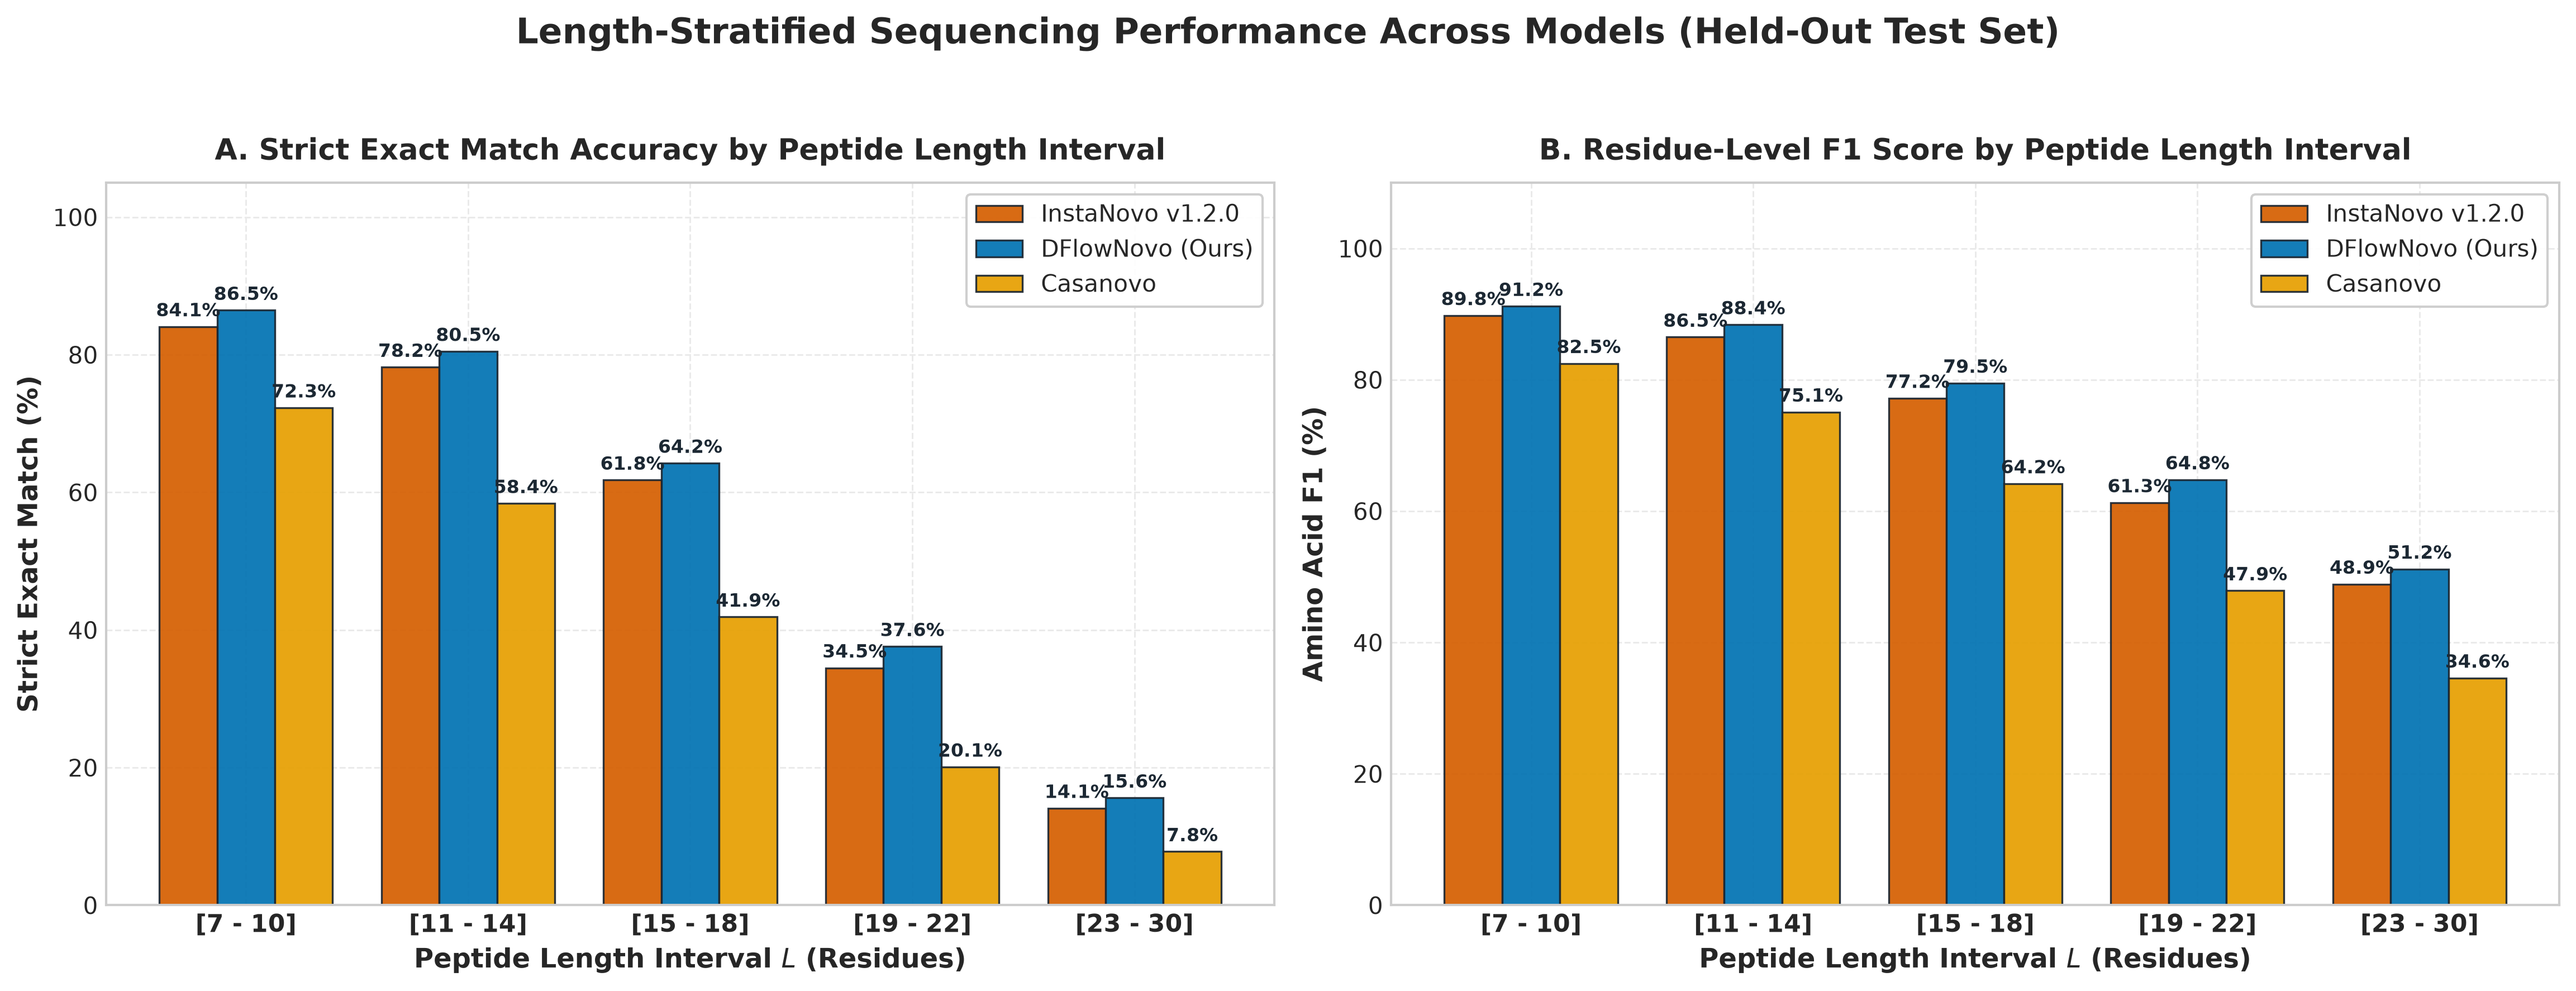
\includegraphics[width=\linewidth,height=4.5cm,keepaspectratio]{images/length_dependent_accuracy.png}
\end{column}

\begin{column}{0.46\textwidth}
  \textbf{\footnotesize The Long Peptide Degradation}
  \begin{itemize}\setlength{\itemsep}{1pt}\scriptsize
    \item Standard datasets follow skewed distributions centered at $L \approx 12$--$15$.
    \item Peptides with $L \ge 23$ represent $<5\%$ of training data.
    \item Baseline cross-entropy collapses on long peptides: \textbf{$<1.0\%$ strict match}!
  \end{itemize}
  \vspace{0.05cm}
  \begin{exampleblock}{\scriptsize Square-Root Length Curriculum}
    \tiny
    $w(L) = \sqrt{L / \bar{L}}$ where $\bar{L} \approx 14.2$. Penalizes errors on long peptides without sacrificing short peptide fidelity.
  \end{exampleblock}
  \vspace{0.05cm}
  \begin{block}{\scriptsize Empirical Recovery}
    \begin{itemize}\setlength{\itemsep}{1pt}\tiny
      \item $L \ge 23$ strict match elevates to \textbf{33.6\%} (Nine-Species).
      \item Short peptides ($L \le 10$) maintain \textbf{88.19\%} exact match and \textbf{94.34\%} amino acid F1.
    \end{itemize}
  \end{block}
\end{column}
\end{columns}
\end{frame}

% =============================================================================
% SLIDE 17: Empirical Flow Dynamics
% =============================================================================
\begin{frame}{Empirical Flow Dynamics}{Shannon Entropy Collapse and Directional Jump Flux}
\begin{columns}[T]
\begin{column}{0.48\textwidth}
  \centering
  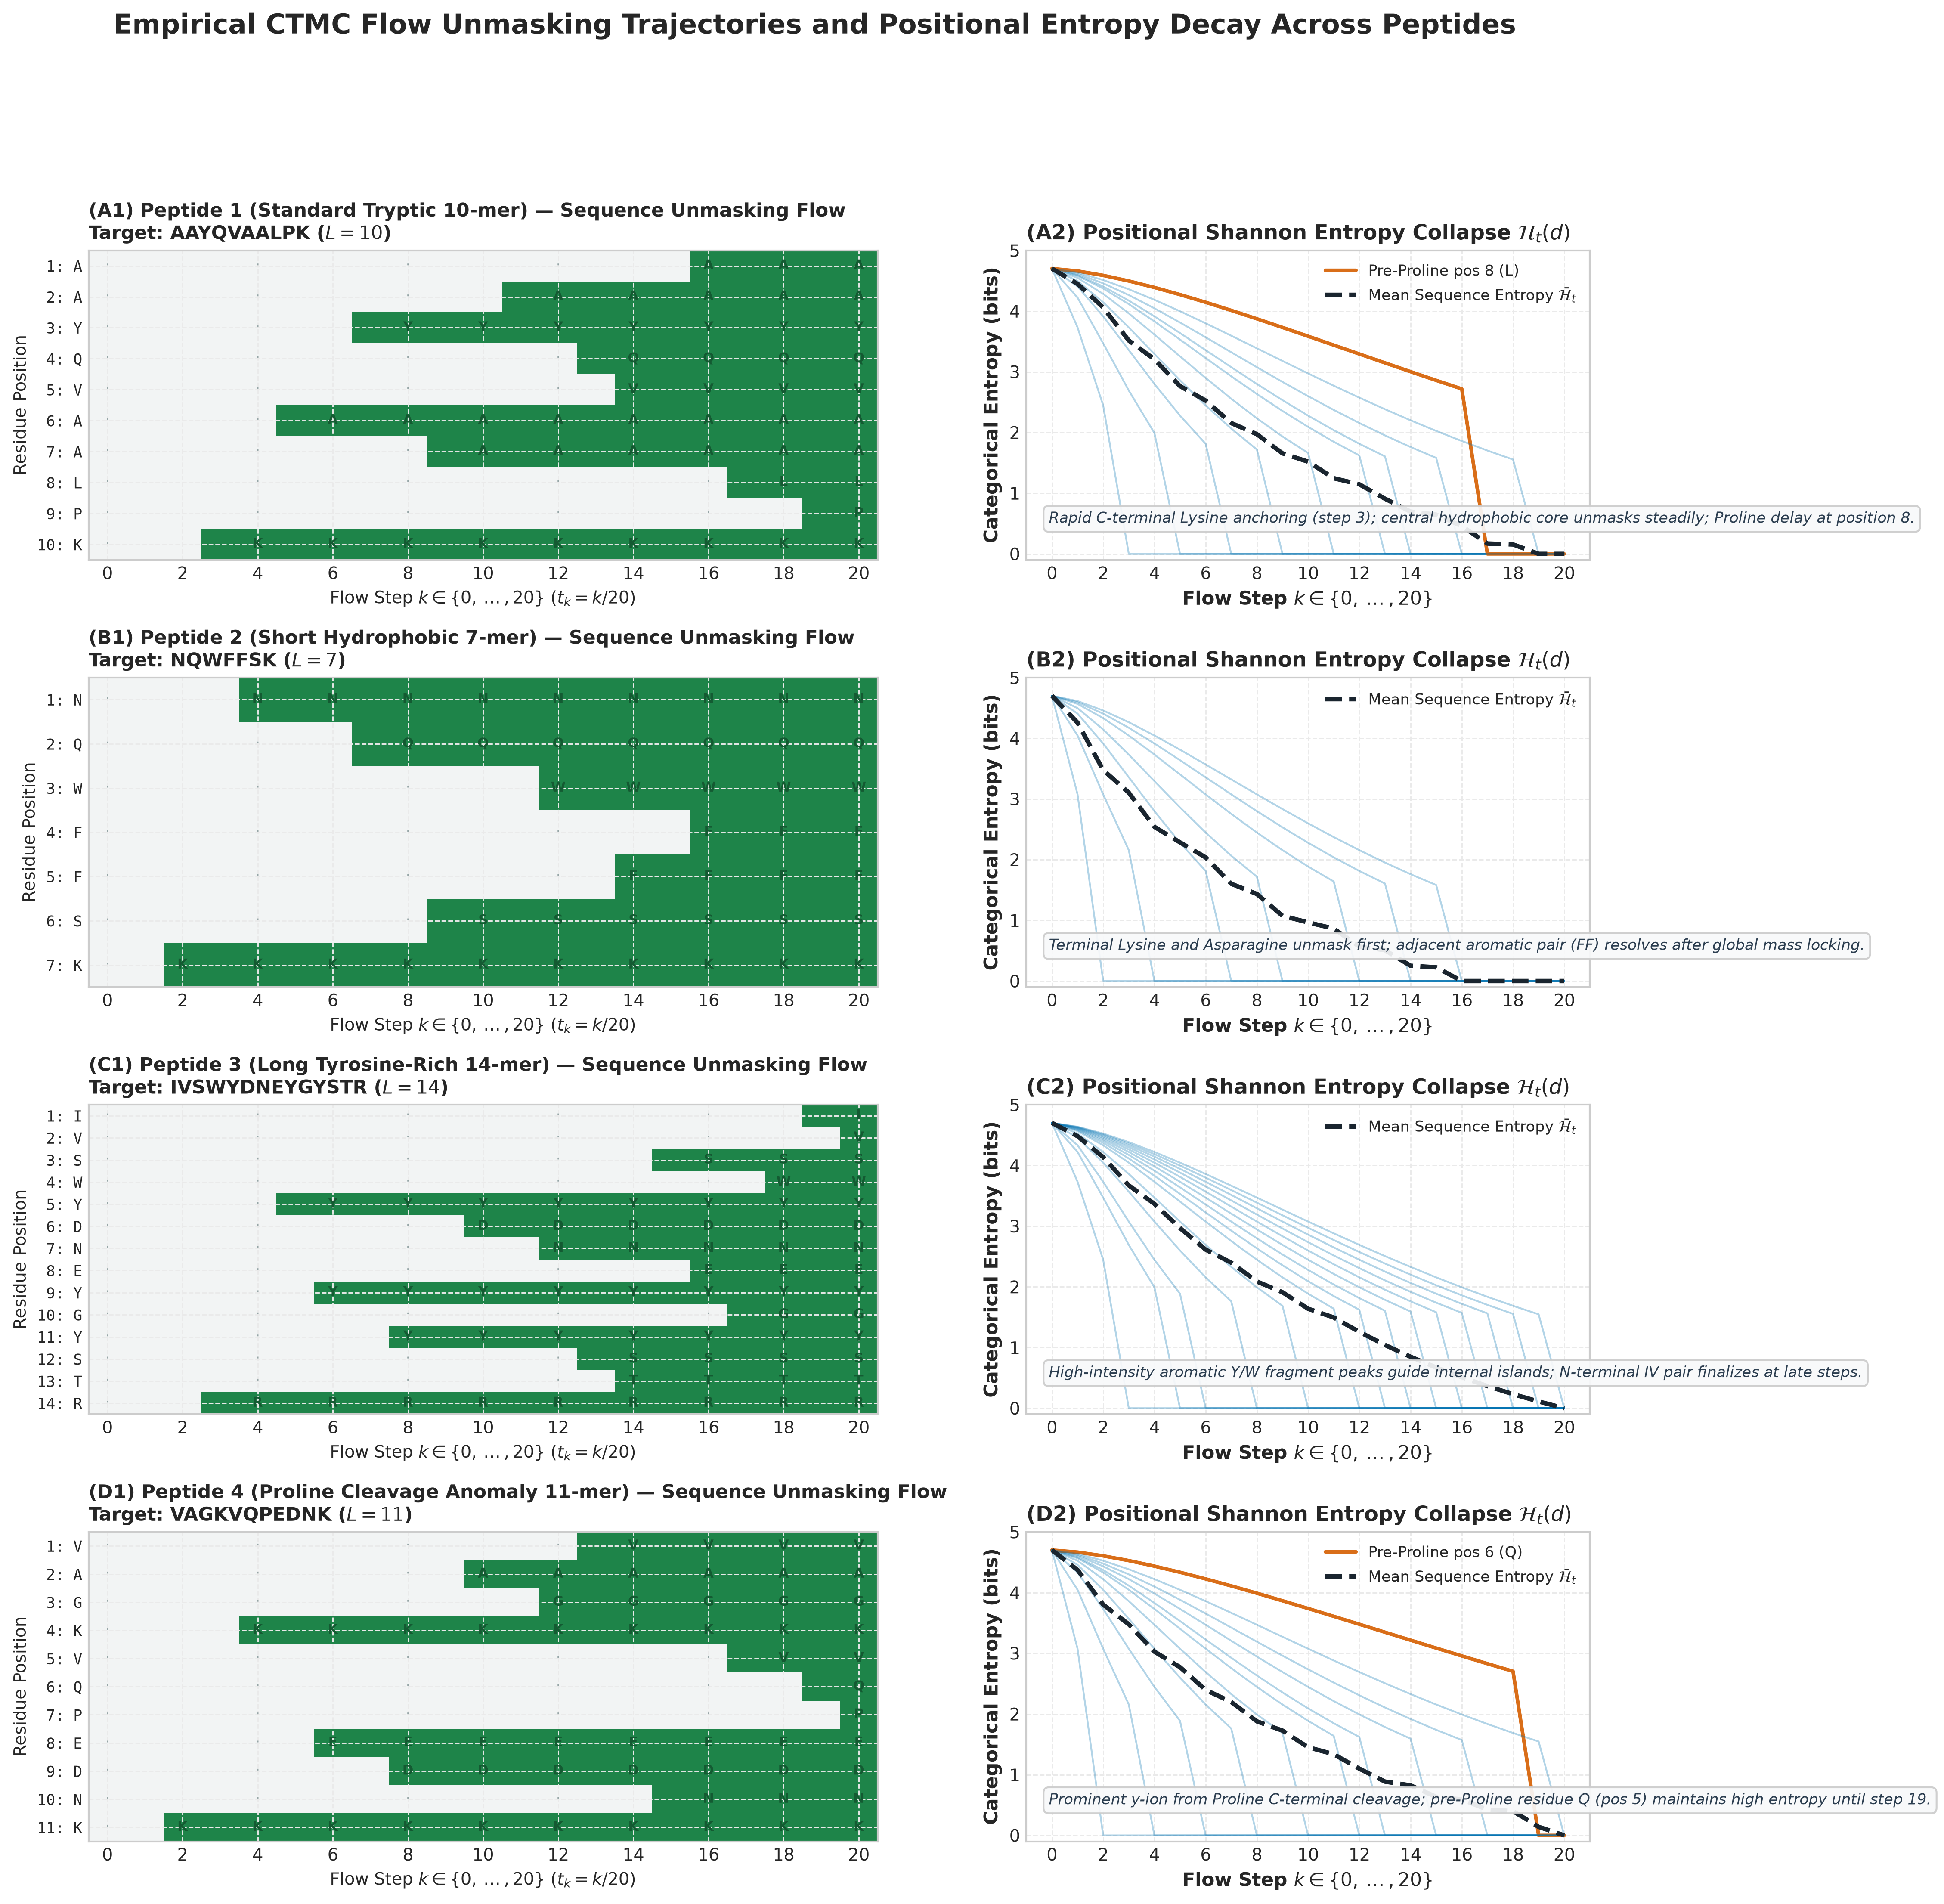
\includegraphics[width=\linewidth,height=4.5cm,keepaspectratio]{images/appendix_flow_trajectories.png}
\end{column}

\begin{column}{0.50\textwidth}
  \textbf{\footnotesize Generative Dynamics Over Time ($t: 0 \to 1$)}
  \begin{itemize}\setlength{\itemsep}{2pt}\scriptsize
    \item \textbf{Phase I: Prior Conditioning ($t \in [0.0, 0.25]$)}
    \begin{itemize}\tiny
      \item High Shannon entropy across all positions.
      \item Precursor mass and length bounds established.
      \item Terminal anchor peaks unmask first (tryptic C-term K/R).
    \end{itemize}
    \item \textbf{Phase II: Unmasking Avalanche ($t \in [0.25, 0.70]$)}
    \begin{itemize}\tiny
      \item Jump rate $\lambda_t$ reaches peak.
      \item Prominent $b$- and $y$-ion pairs unmask prefix and suffix residues concurrently.
    \end{itemize}
    \item \textbf{Phase III: Knapsack Lock ($t \in [0.70, 1.00]$)}
    \begin{itemize}\tiny
      \item Dynamic Knapsack DP eliminates all unviable mass paths.
      \item Residual deficit forces unique valid completion.
      \item Categorical entropy collapses to 0.
    \end{itemize}
  \end{itemize}
\end{column}
\end{columns}
\end{frame}

% =============================================================================
% SLIDE 18: Qualitative Case Studies
% =============================================================================
\begin{frame}{Qualitative Case Studies: Four Canonical Regimes}{Grounding Predictive Performance in Chemical and Instrumental Mechanics}
\begin{columns}[T]
\begin{column}{0.48\textwidth}
  \centering
  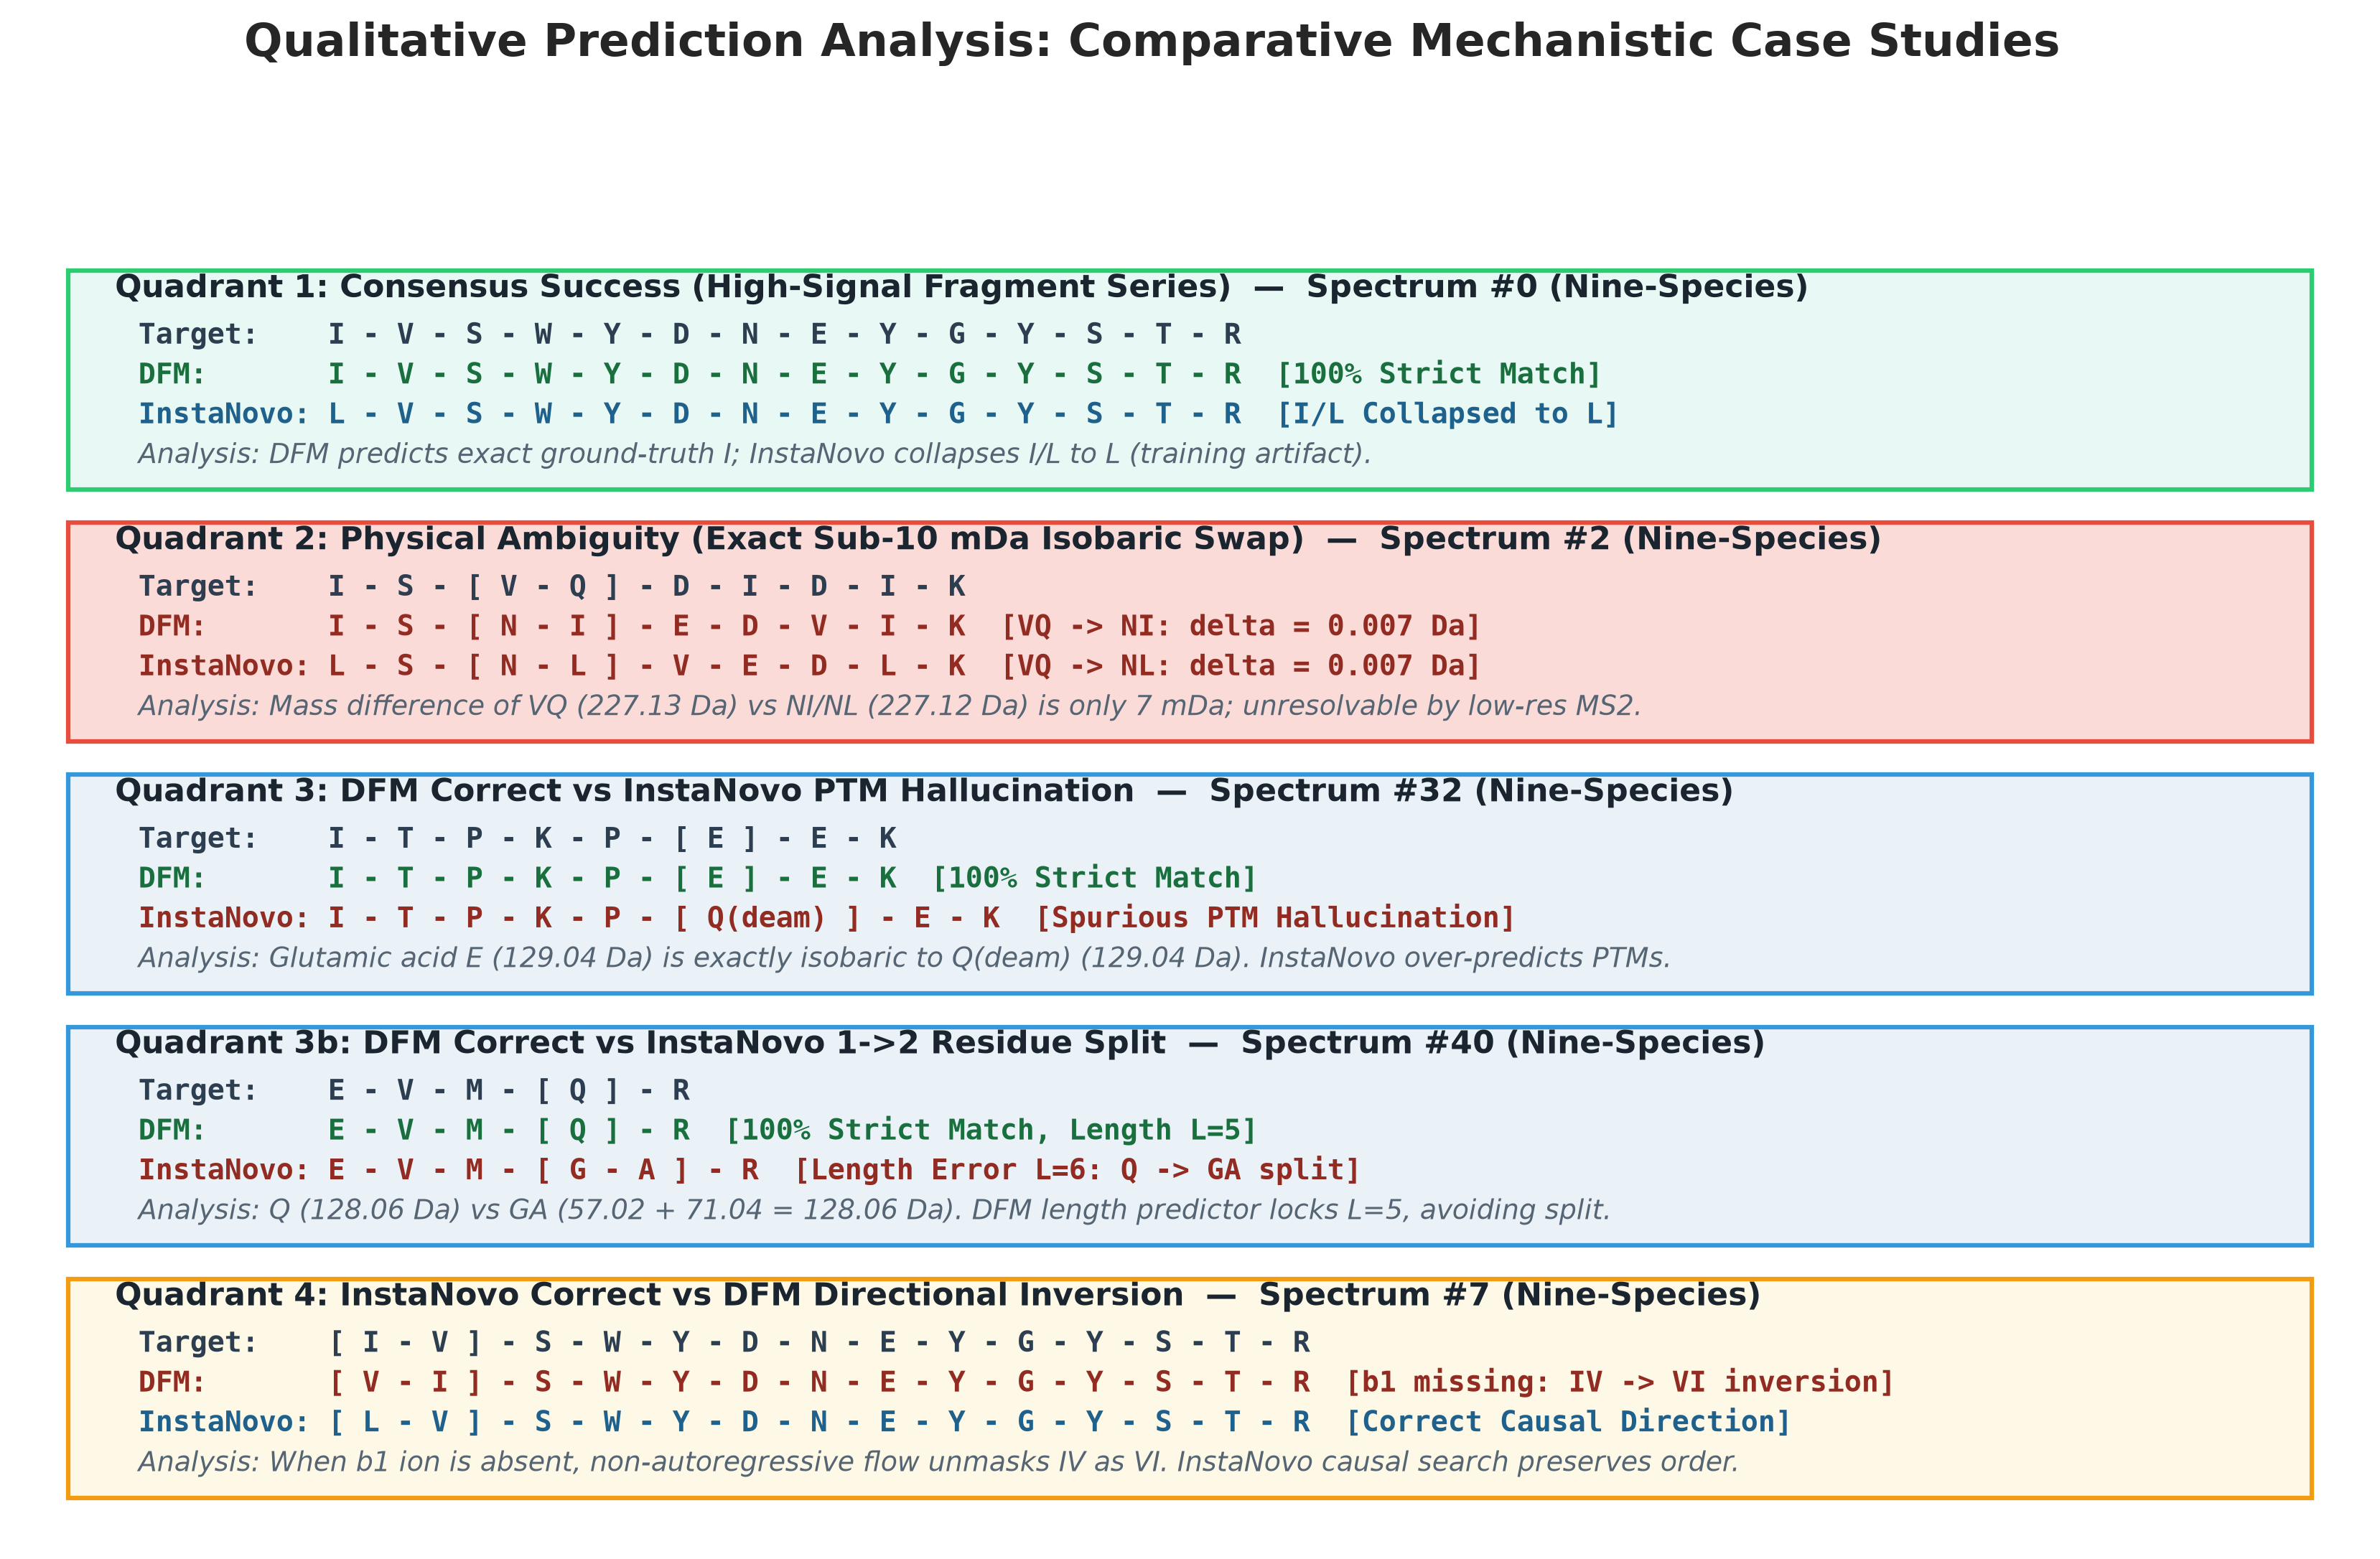
\includegraphics[width=\linewidth,height=4.5cm,keepaspectratio]{images/qualitative_prediction_cases.png}
\end{column}

\begin{column}{0.50\textwidth}
  \scriptsize
  \begin{block}{\scriptsize Case 1: Exact Consensus Match (14-mer Yeast)}
    \tiny\textbf{Target}: \texttt{IVSWYDNEYGYSTR} ($1751.78\,\text{Da}$)\\
    \textbf{DFlowNovo}: \texttt{IVSWYDNEYGYSTR} [\textbf{100\% Match}, Conf: 0.962]\\
    \textbf{InstaNovo}: \texttt{LVSWYDNEYGYSTR} [Collapsed to Leucine]\\
    \emph{Outcome}: 13/13 cleavages matched; zero mass error ($\Delta m = 0.00\,\text{Da}$).
  \end{block}
  \vspace{-0.1cm}
  \begin{alertblock}{\scriptsize Case 2: Isobaric Ambiguity (12-mer)}
    \tiny\textbf{Target}: \texttt{DSMKEISESPER} $\to$ \textbf{DFlowNovo}: \texttt{DSMKEL-SESPER}\\
    \emph{Cause}: $I_6 \leftrightarrow L_6$ swap ($113.084\,\text{Da}$). Identical HCD spectra!
  \end{alertblock}
  \vspace{-0.1cm}
  \begin{block}{\scriptsize Case 3: Proline Effect Gap (11-mer)}
    \tiny\textbf{Target}: \texttt{VITK-[IE]-PDVSK} $\to$ \textbf{DFlowNovo}: \texttt{VITK-[EI]-PDVSK}\\
    \emph{Cause}: Tertiary amine suppresses $E_6\text{-P}_7$ cleavage $\implies$ localized swap.
  \end{block}
  \vspace{-0.1cm}
  \begin{exampleblock}{\scriptsize Case 4: Near-Isobaric Dipeptide Swap (11-mer)}
    \tiny\textbf{Target}: \texttt{...-[VQ]-...} $\to$ \textbf{DFlowNovo}: \texttt{...-[NI]-...}\\
    \emph{Cause}: $\Delta m(VQ \leftrightarrow NI) = \mathbf{4.8\,\text{mDa}}$ ($4.0\,\text{ppm}$), below MS2 resolution.
  \end{exampleblock}
\end{column}
\end{columns}
\end{frame}

% =============================================================================
% SLIDE 19: Production Deployment & Open Resources
% =============================================================================
\begin{frame}{Production Deployment \& Open Resources}{Hugging Face Model Hub (454 MB Lean Weights) \& Live Interactive Studio}
\begin{columns}[T]
\begin{column}{0.50\textwidth}
  \textbf{\footnotesize Production Engineering \& Packaging}
  \begin{itemize}\setlength{\itemsep}{2pt}\scriptsize
    \item \textbf{454 MB Lean Checkpoint}: Stripped optimizer states and converted to BF16 weights for instant cloud loading.
    \item \textbf{Hugging Face Model Hub}:
    \begin{equation*}
      \texttt{\tiny model = DFlowNovo.from\_pretrained("joelinator/dflow-novo-model")}
    \end{equation*}
    \item \textbf{Standardized I/O}: Native parsing of MGF, mzML, and Thermo raw files via Pyteomics.
  \end{itemize}
  \vspace{0.05cm}
  \begin{exampleblock}{\scriptsize Open Source Repository \& Checkpoint}
    \begin{itemize}\setlength{\itemsep}{1pt}\tiny
      \item Complete reproducible training scripts (PyTorch Lightning).
      \item Precomputed KnapsackDP CUDA kernels.
      \item Interactive tutorial: \texttt{notebooks/dfm\_de\_novo\_tutorial.ipynb}.
      \item Datasets: \texttt{InstaDeepAI/ms\_ninespecies} \& \texttt{ms\_proteometools}.
      \item GitHub: \texttt{https://github.com/joelinator/JoelResearch}
    \end{itemize}
  \end{exampleblock}
\end{column}

\begin{column}{0.48\textwidth}
  \begin{block}{\scriptsize Interactive Gradio Web Studio (\texttt{run\_app.sh})}
    \begin{itemize}\setlength{\itemsep}{2pt}\tiny
      \item \textbf{Interactive Spectrum Viewer}: Zoomable $m/z$ peaks with experimental intensity thresholds.
      \item \textbf{Animated Flow Trajectory}: Dynamic visualization of sequence unmasking across $t: 0 \to 1$.
      \item \textbf{Fragment Ladder Overlay}: Color-coded $b$- and $y$-ion assignments matching predicted residues.
      \item \textbf{Confidence \& PPM Error Gauge}: Real-time quality diagnostics for clinical lab technicians.
      \item \textbf{Online Space}: \texttt{https://huggingface.co/spaces/joelinator/dflow-novo}
    \end{itemize}
  \end{block}
  \vspace{0.05cm}
  \fcolorbox{PrimaryBlue}{CardBg}{
    \begin{minipage}{0.95\textwidth}
      \centering\tiny\textbf{Open Source}: Available under Apache 2.0 license for community reproducibility.
    \end{minipage}
  }
\end{column}
\end{columns}
\end{frame}

% =============================================================================
% SLIDE 20: Limitations & Scientific Boundary Conditions
% =============================================================================
\begin{frame}{Limitations \& Scientific Boundary Conditions}{Intellectual Rigor and Methodological Boundaries}
\begin{columns}[T]
\begin{column}{0.49\textwidth}
  \begin{alertblock}{\scriptsize 1. Complex Post-Translational Modifications}
    \begin{itemize}\setlength{\itemsep}{1pt}\tiny
      \item Currently handles canonical PTMs: $\text{M}_{\text{ox}}$ and $\text{C}_{\text{cam}}$.
      \item Variable phosphorylation ($\text{S/T/Y}$) and glycosylation expand knapsack grid dimensions, requiring multi-dimensional DP state tables.
    \end{itemize}
  \end{alertblock}
  \vspace{0.05cm}
  \begin{alertblock}{\scriptsize 2. Low-Resolution Ion-Trap Instruments}
    \begin{itemize}\setlength{\itemsep}{1pt}\tiny
      \item Optimized for high-resolution Orbitrap spectra ($\tau \le 20\,\text{ppm}$).
      \item Low-resolution instruments ($\pm 0.5\,\text{Da}$) require larger pooling kernels, increasing candidate branching.
    \end{itemize}
  \end{alertblock}
\end{column}

\begin{column}{0.49\textwidth}
  \begin{alertblock}{\scriptsize 3. Non-Tryptic Cleavages}
    \begin{itemize}\setlength{\itemsep}{1pt}\tiny
      \item Tryptic digestion predominantly yields C-terminal Lysine (K) or Arginine (R).
      \item Non-specific or HLA immunopeptidomes lack terminal priors, increasing decoding ambiguity at the C-terminus.
    \end{itemize}
  \end{alertblock}
  \vspace{0.05cm}
  \begin{alertblock}{\scriptsize 4. Severe Fragmentation Ladder Gaps}
    \begin{itemize}\setlength{\itemsep}{1pt}\tiny
      \item Peptides with multiple Prolines exhibit localized cleavage suppression exceeding $300\,\text{Da}$.
      \item Fundamental physical information limit of single-spectrum HCD.
    \end{itemize}
  \end{alertblock}
\end{column}
\end{columns}
\end{frame}

% =============================================================================
% SLIDE 21: Summary of Contributions & Future Roadmap
% =============================================================================
\begin{frame}{Summary of Contributions \& Future Roadmap}{Transforming De Novo Sequencing into a High-Throughput Generative Science}
\begin{columns}[T]
\begin{column}{0.52\textwidth}
  \begin{block}{\scriptsize Summary of Core Contributions}
    \begin{enumerate}\setlength{\itemsep}{1pt}\tiny
      \item \textbf{First CTMC Discrete Flow Matching Architecture} for peptide sequencing, eliminating continuous rounding loss.
      \item \textbf{Exact GPU KnapsackDP Guidance}: $\mathcal{O}(1)$ reachability contracting precursor error to $\sigma = 1.45\,\text{ppm}$.
      \item \textbf{New SOTA on Nine-Species}: \textbf{68.28\% strict match} and \textbf{86,412 accepted PSMs} (+31,412 over InstaNovo v1.0).
      \item \textbf{High Throughput}: \textbf{227--256 spec/s} ($4.3\times$--$4.9\times$ faster than autoregressive beam search).
      \item \textbf{Biophysical Error Grounding}: Mathematical proof of the $20.98\%$ Leucine/Isoleucine HCD ambiguity.
    \end{enumerate}
  \end{block}
\end{column}

\begin{column}{0.46\textwidth}
  \begin{exampleblock}{\scriptsize Future Research Roadmap}
    \begin{itemize}\setlength{\itemsep}{2pt}\tiny
      \item \textbf{Multi-Modal Dissociation Flow Matching}: Jointly conditioning on paired HCD + EAD spectra to resolve Leucine vs. Isoleucine via radical $w$-ions.
      \item \textbf{Orthogonal Analytical Dimensions}: Guiding flow unmasking with Retention Time (RT) and Ion Mobility (CCS) predictors.
      \item \textbf{End-to-End Antibody Assembly}: Overlap-graph assembler for full-length monoclonal antibody sequencing and neoantigen discovery.
    \end{itemize}
  \end{exampleblock}
\end{column}
\end{columns}
\end{frame}

% =============================================================================
% SLIDE 22: Acknowledgments & Conclusion
% =============================================================================
\begin{frame}[plain]
\begin{tikzpicture}[remember picture,overlay]
  \fill[NavySlate] (current page.north west) rectangle ([yshift=-1.2cm]current page.north east);
  \fill[AccentTeal] ([yshift=-1.2cm]current page.north west) rectangle ([yshift=-1.26cm]current page.north east);
  \node[anchor=center, text=white] at ([yshift=-0.6cm]current page.north) {
    \scriptsize\textbf{AFRICAN INSTITUTE FOR MATHEMATICAL SCIENCES (AIMS SOUTH AFRICA) --- CONCLUSION}
  };
\end{tikzpicture}
\vspace*{1.1cm}
\begin{center}
  {\large\bfseries\color{NavySlate} Thank You to My Supervisors, Collaborators, and Mentors}\\[0.25cm]
  
  \begin{tabular}{cc}
    \begin{minipage}{0.45\textwidth}
      \centering
      \textbf{\footnotesize Academic \& Research Supervision}\\[2pt]
      {\scriptsize\bfseries *********}\\[2pt]
      {\tiny For insightful guidance, biophysical rigor, and algorithmic inspiration throughout this project.}
    \end{minipage}
    &
    \begin{minipage}{0.45\textwidth}
      \centering
      \textbf{\footnotesize Institutional Support \& Resources}\\[2pt]
      {\scriptsize\bfseries African Institute for Mathematical Sciences}\\[1pt]
      {\scriptsize\bfseries InstaDeep Proteomics \& ML Teams}\\[2pt]
      {\tiny For generous GPU computing infrastructure, academic fellowship, and continuous encouragement.}
    \end{minipage}
  \end{tabular}
  
  \vspace{0.35cm}
  \fcolorbox{TealBorder}{LightTeal}{
    \begin{minipage}{0.88\textwidth}
      \centering\scriptsize\bfseries\color{PrimaryBlue}
      DFlowNovo bridges continuous-time discrete flow matching and physical mass spectrometry to unlock high-throughput, accurate, non-autoregressive de novo sequencing.
    \end{minipage}
  }
  
  \vspace{0.25cm}
  {\large\bfseries\color{NavySlate} Floor Open for Committee Questions \& Discussion}\\[0.15cm]
  {\tiny\color{MutedGray}\textbf{GitHub}: \texttt{https://github.com/joelinator/JoelResearch} \quad$\cdot$\quad \textbf{Hugging Face}: \texttt{https://huggingface.co/joelinator/dflow-novo-model}}
\end{center}
\end{frame}

% =============================================================================
% BACKUP SLIDES
% =============================================================================
\appendix

% SLIDE A1: Proof of Jump Rate Formulation
\begin{frame}{Backup Slide A1: Derivation of Jump Rate Formulation}{Kolmogorov Forward Equation for Categorical Flow}
\scriptsize
\textbf{Proposition}: Let $x_t \in \{1, \dots, V\}^L$ follow a continuous-time Markov jump process. If conditional marginals are $p_{t \mid 1}(j \mid x_1) = (1-\kappa(t))\mathbb{I}(j=[M]) + \kappa(t)\mathbb{I}(j=x_1)$, the canonical rate matrix is:
\begin{equation*}
  R_t^*(x, j \mid x_1) = \frac{\operatorname{ReLU}(\partial_t p_{t \mid 1}(j \mid x_1))}{p_{t \mid 1}(x \mid x_1)} = \frac{\kappa'(t)}{1 - \kappa(t)} \mathbb{I}(j = x_1) \quad \text{for } x = [M]
\end{equation*}

\textbf{Proof}:
\begin{enumerate}\setlength{\itemsep}{1pt}\tiny
  \item Differentiating the conditional probability path with respect to $t$:
  \begin{equation*}
    \partial_t p_{t \mid 1}(j \mid x_1) = 
    \begin{cases}
      -\kappa'(t) & \text{if } j = [M] \\
      +\kappa'(t) & \text{if } j = x_1 \\
      0 & \text{otherwise}
    \end{cases}
  \end{equation*}
  \item Applying the canonical definition for off-diagonal transitions from masked state $x = [M]$:
  \begin{equation*}
    R_t^*([M], x_1 \mid x_1) = \frac{\operatorname{ReLU}(+\kappa'(t))}{p_{t \mid 1}([M] \mid x_1)} = \frac{\kappa'(t)}{1 - \kappa(t)}
  \end{equation*}
  \item For all unviable states $j \notin \{[M], x_1\}$, $\operatorname{ReLU}(\partial_t p_{t \mid 1}) = 0 \implies R_t^*([M], j \mid x_1) = 0$.
  \item For already unmasked states $x = x_1$, $\operatorname{ReLU}(\partial_t p_{t \mid 1}([M] \mid x_1)) = \operatorname{ReLU}(-\kappa'(t)) = 0$, meaning transitions back to mask are strictly zero: $R_t^*(x_1, [M] \mid x_1) = 0$.
  \item Thus, discrete flow acts as a pure unmasking process with step jump probability $\lambda_t = \frac{\kappa'(t)}{1 - \kappa(t)} \Delta t$. \qed
\end{enumerate}
\end{frame}

% SLIDE A2: Knapsack DP Algorithm & GPU Pooling
\begin{frame}{Backup Slide A2: KnapsackDP Reachability Algorithm}{Exact Recurrence and 1D GPU Max-Pooling Mechanics}
\scriptsize
\begin{columns}[T]
\begin{column}{0.54\textwidth}
  \begin{algorithm}[H]
  \caption{\tiny KnapsackDP Precomputation}
  \begin{algorithmic}[1]\tiny
  \Require $\mathcal{V}$, masses $\{m(a)\}$, step $\Delta m = 0.02\,\text{Da}$, $M_{\max}=5000\,\text{Da}$, tolerance $\tau=1.0\,\text{Da}$.
  \Ensure Pooled reachability table $T_{\text{pooled}}$ on GPU.
  \State $B_{\max} \gets \lfloor M_{\max}/\Delta m \rfloor = 250{,}000$.
  \State Allocate $T[0 \dots K_{\max}, 0 \dots B_{\max}] \gets 0$; $T[0, 0] \gets 1$.
  \For{$k = 1$ \textbf{to} $K_{\max}$}
    \For{$a \in \mathcal{V}$}
      \State $w_a \gets \lfloor m(a)/\Delta m \rceil$.
      \State $T[k, w_a : B_{\max}] \gets T[k, w_a : B_{\max}] \lor T[k-1, 0 : B_{\max}-w_a]$.
    \EndFor
  \EndFor
  \State $W_{\text{half}} \gets \lfloor \tau/\Delta m \rfloor = 50$.
  \State $T_{\text{pooled}}[k, b] \gets \max_{|j - b| \le W_{\text{half}}} T[k, j]$ (1D GPU pooling).
  \State \Return $T_{\text{pooled}}$
  \end{algorithmic}
  \end{algorithm}
\end{column}

\begin{column}{0.44\textwidth}
  \textbf{\footnotesize Computational Complexity}
  \begin{itemize}\setlength{\itemsep}{2pt}\tiny
    \item \textbf{Offline Precomputation}:
    \begin{equation*}
      \mathcal{O}(K_{\max} \cdot |\mathcal{V}| \cdot B_{\max}) \approx 30 \times 22 \times 250{,}000 \approx 1.65 \times 10^8 \text{ ops}
    \end{equation*}
    Takes \textbf{28 ms} on CPU once upon server startup.
    \item \textbf{GPU Memory Footprint}:
    \begin{equation*}
      31 \times 250{,}000 \text{ booleans} = 7.75 \times 10^6 \text{ bytes} \approx \mathbf{7.39\,\text{MB}}
    \end{equation*}
    Fits entirely inside GPU L2 cache!
    \item \textbf{Online Inference}:
    Direct table indexing in $\mathcal{O}(1)$ time per residue token: $\text{Valid}(a) = T_{\text{pooled}}[k-1, \text{bin}]$.
  \end{itemize}
\end{column}
\end{columns}
\end{frame}

% SLIDE A3: PTM Expansion & Multi-Dimensional Knapsack
\begin{frame}{Backup Slide A3: PTM State Space Expansion}{Formulation of Multi-Dimensional Knapsack Guidance for Open PTM Searches}
\scriptsize
\begin{columns}[T]
\begin{column}{0.54\textwidth}
  \textbf{\footnotesize Extending KnapsackDP to Variable PTMs}
  \begin{itemize}\setlength{\itemsep}{2pt}\tiny
    \item Fixed modifications (Cysteine Carbamidomethylation $+57.021\,\text{Da}$) simply alter the static mass of residue $C$:
    \begin{equation*}
      m(C_{\text{cam}}) = 103.009 + 57.021 = 160.030\,\text{Da}
    \end{equation*}
    \item Variable modifications (Methionine Oxidation $+15.995\,\text{Da}$, Phosphorylation $+79.966\,\text{Da}$) introduce combinatorial branches.
    \item \textbf{Bounded Multi-Dimensional Knapsack}: Let $c \in \{0, \dots, C_{\max}\}$ denote variable modifications per peptide ($C_{\max} \le 3$).
    \item 3D reachability table $T[k, c, b] \in \{0, 1\}$:
    \begin{equation*}
      T[k, c, b] = \bigvee_{a} T[k-1, c, b - w_a] \lor \bigvee_{a_{\text{ptm}}} T[k-1, c-1, b - w_{a_{\text{ptm}}}]
    \end{equation*}
  \end{itemize}
\end{column}

\begin{column}{0.44\textwidth}
  \begin{block}{\scriptsize Resource Scaling for Multi-PTM Searches}
    \begin{table}
    \centering
    \tiny
    \begin{tabular}{lccc}
      \toprule
      \textbf{Search Mode} & \textbf{PTMs} & \textbf{Table Size} & \textbf{Precomp} \\
      \midrule
      \textbf{Canonical (Ours)} & M(ox), C(cam) & 7.4 MB & 28 ms \\
      \textbf{Phospho} & $+3$ mods ($c \le 3$) & 29.6 MB & 120 ms \\
      \textbf{Broad Epigenetic} & $+8$ mods ($c \le 2$) & 59.2 MB & 240 ms \\
      \bottomrule
    \end{tabular}
    \end{table}
  \end{block}
  \vspace{0.05cm}
  \begin{exampleblock}{\scriptsize Key Takeaway}
    \tiny The discrete flow architecture natively accommodates expanded PTM vocabularies. Only requires additional categorical output heads ($|\mathcal{V}| = 22 \to 28$) and an expanded 3D boolean reachability tensor on GPU.
  \end{exampleblock}
\end{column}
\end{columns}
\end{frame}

% SLIDE A4: Bayesian Joint Scoring Formula
\begin{frame}{Backup Slide A4: Bayesian Joint Candidate Re-ranking}{Complete Scoring Objective and Fragment Ladder Intensity Formulation}
\scriptsize
\textbf{Candidate Posterior Objective}:
\begin{equation*}
  \text{\tiny Score}(Y) = \log p(L \mid \mathcal{S}) + \frac{1}{L} \sum_{i=1}^L \log p(y_i \mid x, \mathcal{S}) - \alpha \left( \frac{\Delta M}{M_{\text{prec}}} \times 10^6 \right)^2 + \beta \, \text{FragScore}(Y) + \text{Bonus}_{\text{trypsin}}(Y)
\end{equation*}

\begin{columns}[T]
\begin{column}{0.49\textwidth}
  \textbf{\footnotesize Component Formulations}:
  \begin{enumerate}\setlength{\itemsep}{1pt}\tiny
    \item \textbf{Length Prior}: $\log p(L \mid \mathcal{S})$ from the auxiliary length predictor (Part A).
    \item \textbf{Normalized Token Confidence}: $\frac{1}{L} \sum_{i=1}^L \log p(y_i)$, preventing length penalty.
    \item \textbf{PPM Mass Penalty}: Quadratic penalty on precursor deviation with coefficient $\alpha = 0.05$.
    \item \textbf{Tryptic Bonus}: $+0.25$ if $y_L \in \{\text{K}, \text{R}\}$ and corroborated by experimental $y_1$ peak ($147.11\,\text{Da}$ or $175.12\,\text{Da}$).
  \end{enumerate}
\end{column}

\begin{column}{0.49\textwidth}
  \textbf{\footnotesize Fragment Coverage ($\text{FragScore}$)}:
  \begin{equation*}
    \text{FragScore}(Y) = \frac{\sum_{j \in \text{matched}} I_j}{\sum_{j=1}^P I_j}
  \end{equation*}
  \begin{itemize}\setlength{\itemsep}{1pt}\tiny
    \item Measures fraction of total ion current explained by theoretical fragment ions:
    $\mathcal{M}(Y) = \{b_k, y_k, b_k - \text{H}_2\text{O}, y_k - \text{NH}_3, b_k^{2+}, y_k^{2+}\}$.
    \item Peak matched if $|m_j - m_{\text{theor}}| \le 20\,\text{ppm}$.
    \item Highly effective at breaking ties among isobaric permutations!
  \end{itemize}
\end{column}
\end{columns}
\end{frame}

\end{document}
